\documentclass[letterpaper, 10 pt, conference]{ieeeconf}  % Comment this line out if you need a4paper
%\documentclass[a4paper, 10pt, conference]{ieeeconf}      % Use this line for a4 paper
\IEEEoverridecommandlockouts                              % This command is only needed if
\overrideIEEEmargins                                      % Needed to meet printer requirements.

%%%%%%%%%%%%%%%%%%%%%%%%%%%%%%%%%%%%%%%%%%%%%%%%%%%%%%%%%%%%%%%%%%%%%%%%%%%%%%%%

\usepackage{amsmath}
\usepackage{amssymb}
\usepackage{graphicx}
\usepackage{rotating}
\usepackage{xcolor}
\usepackage{tikz}
\usepackage{pgfplots}

%%%%%%%%%%%%%%%%%%%%%%%%%%%%%%%%%%%%%%%%

\DeclareMathOperator*{\argmin}{arg\,min}
\DeclareMathOperator*{\argmax}{arg\,max}
\DeclareMathOperator*{\vectorize}{vec}

\newcommand{\normal}[2]{\ensuremath{\mathcal{N}\left({{#1}},{{#2}}\right)}}
\newcommand{\trans}[1]{\ensuremath{{#1}^{\mathsf{T}}}}

\newcommand{\e}{\mathbf{e}}
\newcommand{\bb}{\mathbf{k}}
\newcommand{\kL}{\mathbf{k}^L}
\newcommand{\kG}{\mathbf{k}^G}
%\newcommand{\uu^m}{\mathbf{w}}
\newcommand{\x}{\mathbf{x}}
\newcommand{\y}{\mathbf{y}}
\newcommand{\uu}{\mathbf{u}}
\newcommand{\vv}{\mathbf{v}}
\newcommand{\timestep}{s}

\newcommand{\fixme}[1]{\textbf{FIXME: {#1}}}
\newcommand{\new}[1]{\color{red} {#1}}

\definecolor{darkgreen}{RGB}{0,127,0}

%%%%%%%%%%%%%%%%%%%%%%%%%%%%%%%%%%%%%%%%%%%%%%%%%%%%%%%%%%%%%%%%%%%%%%%%%%%%%%%%

\begin{filecontents}{paper.bib}
@inproceedings{wan2000unscented,
  title={The unscented Kalman filter for nonlinear estimation},
  author={Wan, Eric A and Van Der Merwe, Rudolph},
  booktitle={Adaptive Systems for Signal Processing, Communications, and Control Symposium 2000. AS-SPCC. The IEEE 2000},
  pages={153--158},
  year={2000},
  organization={Ieee}
}

@inproceedings{morelande2006reduced,
  title={Reduced sigma point filtering for partially linear models},
  author={Morelande, Mark R and Ristic, Branko},
  booktitle={2006 IEEE International Conference on Acoustics Speech and Signal Processing Proceedings},
  volume={3},
  pages={III--III},
  year={2006},
  organization={IEEE}
}

@inproceedings{padilla2010adaptive,
  title={An adaptive-covariance-rank algorithm for the unscented Kalman filter},
  author={Padilla, Lauren E and Rowley, Clarence W},
  booktitle={49th IEEE Conference on Decision and Control (CDC)},
  pages={1324--1329},
  year={2010},
  organization={IEEE}
}

@article{wang2010generating,
  title={Generating statistically correct random topologies for testing smart grid communication and control networks},
  author={Wang, Zhifang and Scaglione, Anna and Thomas, Robert J},
  journal={IEEE transactions on Smart Grid},
  volume={1},
  number={1},
  pages={28--39},
  year={2010},
  publisher={IEEE}
}

@inproceedings{hines2010topological,
  title={The topological and electrical structure of power grids},
  author={Hines, Paul and Blumsack, Seth and Sanchez, E Cotilla and Barrows, Clayton},
  booktitle={System Sciences (HICSS), 2010 43rd Hawaii International Conference on},
  pages={1--10},
  year={2010},
  organization={IEEE}
}


@article{schultz2014random,
  title={A random growth model for power grids and other spatially embedded infrastructure networks},
  author={Schultz, Paul and Heitzig, Jobst and Kurths, J{\"u}rgen},
  journal={The European Physical Journal Special Topics},
  volume={223},
  number={12},
  pages={2593--2610},
  year={2014},
  publisher={Springer}
}

@article{ghahremani2011online,
  title={Online state estimation of a synchronous generator using unscented Kalman filter from phasor measurements units},
  author={Ghahremani, Esmaeil and Kamwa, Innocent},
  journal={IEEE Transactions on Energy Conversion},
  volume={26},
  number={4},
  pages={1099--1108},
  year={2011},
  publisher={IEEE}
}

@article{ghahremani2016local,
  title={Local and wide-area pmu-based decentralized dynamic state estimation in multi-machine power systems},
  author={Ghahremani, Esmaeil and Kamwa, Innocent},
  journal={IEEE Transactions on Power Systems},
  volume={31},
  number={1},
  pages={547--562},
  year={2016},
  publisher={IEEE}
}

@article{ghahremani2011dynamic,
  title={Dynamic state estimation in power system by applying the extended Kalman filter with unknown inputs to phasor measurements},
  author={Ghahremani, Esmaeil and Kamwa, Innocent},
  journal={IEEE Transactions on Power Systems},
  volume={26},
  number={4},
  pages={2556--2566},
  year={2011},
  publisher={IEEE}
}

@article{wang2012alternative,
  title={An alternative method for power system dynamic state estimation based on unscented transform},
  author={Wang, Shaobu and Gao, Wenzhong and Meliopoulos, AP Sakis},
  journal={IEEE Transactions on Power Systems},
  volume={27},
  number={2},
  pages={942--950},
  year={2012},
  publisher={IEEE}
}

@article{qing2015decentralized,
  title={Decentralized unscented Kalman filter based on a consensus algorithm for multi-area dynamic state estimation in power systems},
  author={Qing, Xiangyun and Karimi, Hamid Reza and Niu, Yugang and Wang, Xingyu},
  journal={International Journal of Electrical Power \& Energy Systems},
  volume={65},
  pages={26--33},
  year={2015},
  publisher={Elsevier}
}

@article{rigatos2013distributed,
  title={A distributed state estimation approach to condition monitoring of nonlinear electric power systems},
  author={Rigatos, G and Siano, Q and Zervos, N},
  journal={Asian Journal of Control},
  volume={15},
  number={3},
  pages={849--860},
  year={2013},
  publisher={Wiley Online Library}
}

@article{yang2013false,
  title={On false data injection attacks against Kalman filtering in power system dynamic state estimation},
  author={Yang, Qingyu and Chang, Liguo and Yu, Wei},
  journal={Security and Communication Networks},
  year={2013},
  publisher={Wiley Online Library}
}

@incollection{witczak2014unknown,
  title={Unknown Input Observers and Filters},
  author={Witczak, Marcin},
  booktitle={Fault Diagnosis and Fault-Tolerant Control Strategies for Non-Linear Systems},
  pages={19--56},
  year={2014},
  publisher={Springer}
}

@article{bolandhemmat2012solution,
  title={A Solution to the State Estimation Problem of Systems with Unknown Inputs},
  author={Bolandhemmat, Hamidreza and Clark, Christopher and Golnaraghi, Farid},
  journal={Recent Patents on Mechanical Engineering},
  volume={5},
  number={2},
  pages={102--112},
  year={2012},
  publisher={Bentham Science Publishers}
}

@article{yang1988observers,
  title={Observers for linear systems with unknown inputs},
  author={Yang, Fuyu and Wilde, Richard W},
  journal={IEEE transactions on automatic control},
  volume={33},
  number={7},
  pages={677--681},
  year={1988},
  publisher={Institute of Electrical and Electronics Engineers}
}

@inproceedings{amini2015dynamic,
  title={Dynamic load altering attacks in smart grid},
  author={Amini, Sajjad and Mohsenian-Rad, Hamed and Pasqualetti, Fabio},
  booktitle={Innovative Smart Grid Technologies Conference (ISGT), 2015 IEEE Power \& Energy Society},
  pages={1--5},
  year={2015},
  organization={IEEE}
}

@inproceedings{amini2015detecting,
  title={Detecting dynamic load altering attacks: A data-driven time-frequency analysis},
  author={Amini, Sajjad and Pasqualetti, Fabio and Mohsenian-Rad, Hamed},
  booktitle={2015 IEEE International Conference on Smart Grid Communications (SmartGridComm)},
  pages={503--508},
  year={2015},
  organization={IEEE}
}

@article{fang2012smart,
  title={Smart grid�The new and improved power grid: A survey},
  author={Fang, Xi and Misra, Satyajayant and Xue, Guoliang and Yang, Dejun},
  journal={IEEE communications surveys \& tutorials},
  volume={14},
  number={4},
  pages={944--980},
  year={2012},
  publisher={IEEE}
}

@article{wang2009cascade,
  title={Cascade-based attack vulnerability on the US power grid},
  author={Wang, Jian-Wei and Rong, Li-Li},
  journal={Safety Science},
  volume={47},
  number={10},
  pages={1332--1336},
  year={2009},
  publisher={Elsevier}
}

@article{rosas2007topological,
  title={Topological vulnerability of the European power grid under errors and attacks},
  author={Rosas-Casals, Marti and Valverde, Sergi and Sol{\'e}, Ricard V},
  journal={International Journal of Bifurcation and Chaos},
  volume={17},
  number={07},
  pages={2465--2475},
  year={2007},
  publisher={World Scientific}
}

@article{albert2004structural,
  title={Structural vulnerability of the North American power grid},
  author={Albert, R{\'e}ka and Albert, Istv{\'a}n and Nakarado, Gary L},
  journal={Physical review E},
  volume={69},
  number={2},
  pages={025103},
  year={2004},
  publisher={APS}
}

@Article{FRL1,
author = {A.~Molina-Garcia� and F.~Bouffard and D.~S.~Kirschen},
title = {Decentralized Demand-Side Contribution to Primary Frequency Control},
journal = {IEEE Trans. on Power Systems},
volume = 26,
number = 1,
pages = {411-419},
month = feb,
year = 2011
}

@Article{FRL2,
author = {J.~A.~Short and D.~G.~Infield and L.~L.~Freris},
title = {Stabilization of Grid Frequency Through Dynamic Demand Control},
journal = {IEEE Trans. on Power Systems},
volume = 22,
number = 3,
pages = {1284-1293},
month = aug,
year = 2007
}

@Article{FRL3,
author = {C.~Zhao and U.~Topcu and S.~H.~Low},
title = {Optimal Load Control via Frequency Measurement and Neighborhood Area Communication},
journal = {IEEE Trans. on Power Systems},
volume = 28,
number = 4,
pages = {3576-3587},
month = nov,
year = 2013
}

@inproceedings{Pasqualetti2012,
  title={Cyber-physical security via geometric control: Distributed monitoring and malicious attacks},
  author={Pasqualetti, Fabio and D{\"o}rfler, Florian and Bullo, Francesco},
  booktitle={2012 IEEE 51st IEEE Conference on Decision and Control (CDC)},
  pages={3418--3425},
  year={2012},
  organization={IEEE}
}

@inproceedings{Demarco1996,
  title={The potential for malicious control in a competitive power systems environment},
  author={DeMarco, Christopher L and Sariashkar, JV and Alvarado, Fernando},
  booktitle={Control Applications, 1996., Proceedings of the 1996 IEEE International Conference on},
  pages={462--467},
  year={1996},
  organization={IEEE}
}

@article{Mohsenian-Rad2010,
  title={Distributed internet-based load altering attacks against smart power grids},
  author={Mohsenian-Rad, Amir-Hamed and Leon-Garcia, Alberto},
  journal={IEEE Transactions on Smart Grid},
  volume={2},
  number={4},
  pages={667--674},
  year={2011},
  publisher={IEEE}
}

@article{Marnerides2014,
  title={Power consumption profiling using energy time-frequency distributions in smart grids},
  author={Marnerides, Angelos K and Smith, Paul and Schaeffer-Filho, Alberto and Mauthe, Andreas},
  journal={IEEE Communications Letters},
  volume={19},
  number={1},
  pages={46--49},
  year={2015},
  publisher={IEEE}
}
\end{filecontents}
\immediate\write18{bibtex paper}

%%%%%%%%%%%%%%%%%%%%%%%%%%%%%%%%%%%%%%%%%%%%%%%%%%%%%%%%%%%%%%%%%%%%%%%%%%%%%%%%


\title{\LARGE \bf
    Detection and Identification of Destabilizing Attacks in Power Systems
}

\author{ Mike Izbicki, Sajjad Amini, Christian Shelton, and Hamed Mohsenian-Rad}
%\author{Albert Author$^{1}$ and Bernard D. Researcher$^{2}$% <-this % stops a space
%\thanks{*This work was not supported by any organization}% <-this % stops a space
%\thanks{$^{1}$Albert Author is with Faculty of Electrical Engineering, Mathematics and Computer Science,
        %University of Twente, 7500 AE Enschede, The Netherlands
        %{\tt\small albert.author@papercept.net}}%
%\thanks{$^{2}$Bernard D. Researcheris with the Department of Electrical Engineering, Wright State University,
        %Dayton, OH 45435, USA
        %{\tt\small b.d.researcher@ieee.org}}%
%}


\begin{document}



\maketitle
\thispagestyle{empty}
\pagestyle{empty}

%%%%%%%%%%%%%%%%%%%%%%%%%%%%%%%%%%%%%%%%%%%%%%%%%%%%%%%%%%%%%%%%%%%%%%%%%%%%%%%%
\begin{abstract}
Destabilizing attacks insert positive feedback into a power system.
This feedback destabilizes the system by changing the power system dynamics,
which can damage equipment.
We propose a method for detecting these attacks before they damage equipment.
We observe that these attacks can be modeled as a reparameterization of the power system's dynamical model.
Our method uses the Unscented Kalman Filter to jointly estimate both the system states and parameters of the attack.
We also propose a low-rank modification to the Kalman filter that improves computational efficiency while maintaining accuracy of detection.
We show empirically that this method successfully identifies complex attacks involving many nodes at once.
\end{abstract}


%%%%%%%%%%%%%%%%%%%%%%%%%%%%%%%%%%%%%%%%%%%%%%%%%%%%%%%%%%%%%%%%%%%%%%%%%%%%%%%%
\section{Introduction}

In this paper, we consider failures in smart power grids caused by destabilizing attacks.
Such attacks can be conducted in different ways.
One of the most common methods for inserting positive feedback is manipulating load consumption by getting feedback from frequency through a simple proportional gain controller.
\fixme{We need to at least list some other attack types.}
This is known as a dynamic load altering attack \cite{}.
We aim to detect the presence of such attacks and identify their type,
e.g. compromised loads in dynamic load altering attacks.

Recent work has made advances on how to detect these attacks \cite{amini2015dynamic,amini2015detecting}.
This prior work has several limitations that are fixed in this paper:
\begin{enumerate}
\item
Prior work is concerned only with identifying attacks on an individual bus.
To identify attacks on the entire system, the method must be run several times separately on every bus.
%This complicates the procedure's implementation and increases computational complexity.
Our method naturally identifies attacks on the entire system considered as a whole.
This reduces the identification time.
\fixme{We need a definition of detection vs identification.}
\item
Prior work can only determine that feedback has been added to the system;
it provides no information about the \emph{sign} nor \emph{magnitude} of the attack.
Our method estimates both.
This information is useful when deciding which countermeasures to take to mitigate the effectiveness of the attack.
%Estimating the magnitude can be important for determining the severity of the attack and deciding the appropriate corrective measures.
\end{enumerate}

\subsection{Related work}
\fixme{This section is basically just a list of possibly related papers.}

%There exist good filtering methods for designing Unknown Input Observers (UIOs).
%\cite{yang1988observers,bolandhemmat2012solution,witczak2014unknown}
%Using one of these methods, we can estimate the control input for our system,
%then apply the previous techniques to detect attacks.
%The UIO technique introduces extra overhead steps, however.
%My technique estimates the attack directly without needing to first estimate the control input.

The unscented Kalman filter has been used before for power system problems.
All of these papers are for estimating the parameters of a single generator connected to an idealized powergrid.
This paper claims that the UKF is better than the EKF for estimating the rotor angle and speed in synchronous generators.
The authors use a fourth-order nonlinear model of a single motor generator with an infinite bus.
No joint estimation is used, and the system is not under attack.
\cite{ghahremani2011online}
This paper uses the EKF-UI algorithm to jointly estimate the parameters of the motor controller and bus loads.
The original system is a fourth-order nonlinear system of the single motor generator.
The system is assumed to be not under attack.
\cite{ghahremani2011dynamic}
Another EKF-UI paper by the same authors.
\cite{ghahremani2016local}

This paper claims that current WAMS monitoring systems of power grids require calculation of a large Jacobian matrix.
They propose using the UKF to avoid the need for a Jacobian, both improving runtime and accuracy.
\cite{wang2012alternative}
This paper claims that using the UKF to monitor realworld power systems is too slow.
They identify two bottlenecks to a centralized monitor.
First, there is a lot of communication required from every node to the monitor.
Second, the monitor must do a lot of computation.
They solve both problems by partitioning the powergrid into disjoint smaller grids,
filtering each grid independently,
and carefully communicating the results between the smaller grids.
A similar technique might be useful to speed up my solution,
but this is a different idea than I had.
\cite{qing2015decentralized}
This paper also does a distributed analysis of realworld power systems as above.
This paper is more similar to our paper because they are specifically looking to detect faults.
They detect faults in a different way.
We have a specific model of the way faults are generated that we are looking to detect by adding new states to the system.
They do not have a specific model, and instead apply a function to the existing states in an attempt to detect faults.
\cite{rigatos2013distributed}


\section{Problem statement}

\begin{figure}
\centering
\begin{tikzpicture}

%\node at (0,10) {};
\node at (0,6) {
    \begin{tikzpicture}
    \begin{axis}
        [ domain=-30:80
        , xmin=-30
        , xmax=80
        , width=0.55\textwidth
        , height=2.5in
        , samples=500
        , xtickmin=1,xtickmax=0,ytickmin=1,ytickmax=0, minor tick num=0, scaled ticks=false, xticklabel=\empty,yticklabel=\empty
        ]
    \draw[ultra thin,opacity=0.2] (axis cs:\pgfkeysvalueof{/pgfplots/xmin},0) -- (axis cs:\pgfkeysvalueof{/pgfplots/xmax},0);
    \draw[ultra thin,opacity=1.2,red] (axis cs:0,\pgfkeysvalueof{/pgfplots/ymin}) -- (axis cs:0,\pgfkeysvalueof{/pgfplots/ymax});
    \addplot[color=blue,mark=none] {(\x>0)*x^(1.75)*sin(deg(x))};
    \end{axis}

    \node at (4.25,3) {\color{blue} $\omega_2$};
    \node at (3.5,4.5) {\color{red} attack initiated};

    \draw[fill=green,draw opacity=0,fill opacity=0.05] (0,1) -- (8.20,1) -- (8.20,3.95) -- (0,3.95);
    \draw[dashed,darkgreen] (0,1) -- (8.2,1);
    \draw[dashed,darkgreen] (8.2,3.95) -- (0,3.95);

    \node at (4.25,1.2) {\color{darkgreen} safe operating range};

    %\node at (
    \end{tikzpicture}
};

\node at (0,0) {
    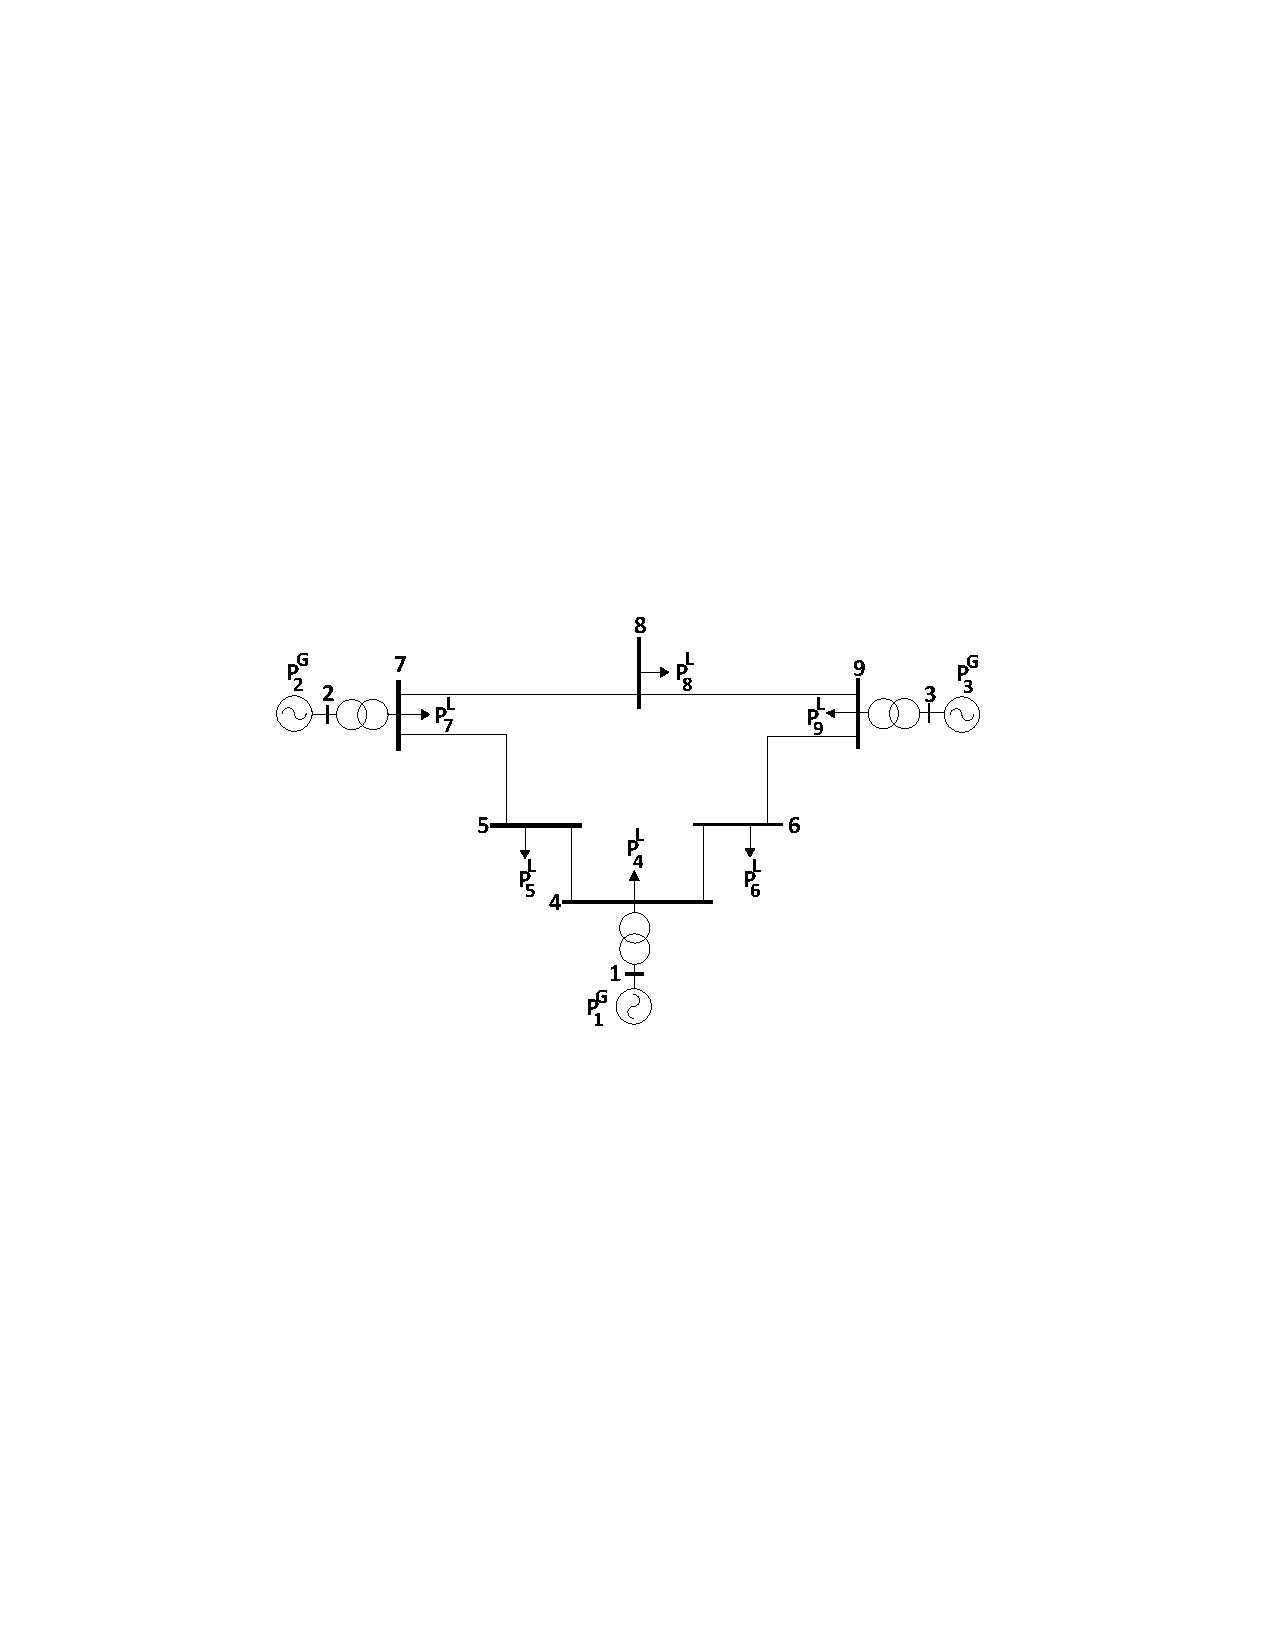
\includegraphics[width=0.43\textwidth]{img/IEEE9}
};

\draw[blue,line width=0.25pt,fill,draw opacity=0.5,fill opacity=0.1]
    (-3.95,0.8) -- (-2.75,0.8) -- (-2.75,1.9) -- (-3.95,1.9) -- cycle;

\draw[dotted,thick] (-3.95,1.9) -- (-4.1,3.6);
\draw[dotted,thick] (-2.75,1.9) -- (4.1,3.6);

\node[draw=red,fill=red,fill opacity=0.05,circle,minimum width=1.5cm] (8) at (0.25,1.6) {};
\node[draw=red,fill=red,fill opacity=0.05,circle,minimum width=1.5cm] (3) at (3.5,1.25) {};
\draw[red,thick,->] (8) to[out=20,in=120] (3);

\end{tikzpicture}
\caption{
    The standard IEEE 9 bus power system under a destabilizing attack.
    The attacker has added a load to bus 8 that gets positive feedback from generator bus 3.
    This causes instabilities throughout the power system.
    The inset shows that generator 2's rotar angle frequency deviation ($\omega_2$).
    During normal operations, $\omega_2$ remains close to 0 because the system is stable.
    The attack adds instability to the system, which causes $\omega_2$ to exceed safe operating levels unless corrective action is taken.
    Our goal is to identify which system buses are compromised so that we can take this corrective action.
}

\label{fig:example}
\end{figure}

Consider a power system with $\mathcal{N} = \mathcal{G} \cup \mathcal{L}$ as the set of buses (i.e. nodes),
where $\mathcal{G}$ and $\mathcal{L}$ are the sets of generator buses and load buses, respectively.
An example is shown in Figure \ref{fig:example}.
The dynamics of this system are commonly modeled using the standard linear power system state space equation
\begin{equation}
\dot\x = A\x + B\uu
,
\label{sys:norm}
\end{equation}
where the state variables and inputs are
\begin{align}
\x
=
\begin{bmatrix} \delta \\ \theta \\ \omega \end{bmatrix}
,
~~~\uu
=
\begin{bmatrix} P^G \\ P^L \end{bmatrix}
.
\end{align}
Here,
$\delta$ is the vector of voltage phase angles at all generator buses,
$\omega$ is the vector of rotor angular frequency deviations at all generator buses,
$\theta$ is the vector of voltage phase angles at all load buses,
$P^L$ is the vector of power consumption at all load buses,
and $P^G$ is the vector of power generation at all generator buses.
Many generators are equipped with Automatic Generation Control (AGC),
which is a system for automatically adjusting the power output in response to the load.
Entries of $P^G$ associated with generators that have AGC are zero.
All other entries are nonzero.
The system dynamics matrices are
%\resizebox{0.4\textwidth}{!}{
\newcommand{\negone}{\scalebox{0.95}{-}1}
\begin{align*}
\hspace{-0.3in}
A
\!\!&=\!\!\!
\begin{bmatrix}
0 & 0 & I
\\
%(D^L)^{-1}H^{LG} & (D^L)^{-1}H^{LL} & -(D^L)^{-1}K^{LG}
(D^L)^{\negone}H^{LG} & (D^L)^{\negone}H^{LL} & 0
\\
-M^{\negone}(K^I\!\!+\!\! H^{GG}) & -M^{\negone}H^{GL} & -M^{\negone}(K^P\!\!\!+\!\!D^G)
\end{bmatrix}
,
%\end{align*}
%\begin{flalign*}
\\
B
%&=
\!\!&=\!\!\!
\begin{bmatrix}
0 & 0
\\
0 & (D^L)^{\negone}
\\
-M^{\negone} & 0
\end{bmatrix}
,
%&
\end{align*}
%}
where
$I$ is the identity matrix of appropriate dimension,
and $M$, $D^G$, and $D^L$ are diagonal matrices with diagonal entries equal to the inertia, damping coefficients of generators, and damping coefficients of loads, respectively.
Matrices $H^{LG}$, $H^{GG}$, $H^{GL}$, and $H^{LL}$ are the imaginary components of the standard system admittance matrix $H^{bus}$.
Specifically,
\begin{align*}
  H^{bus} =
  \begin{bmatrix}
    H^{GG} & H^{GL} \\
    H^{LG} & H^{LL}
  \end{bmatrix}.
\end{align*}
Matrices $K^I$ and $K^P$ are diagonal matrices with diagonal entries equal to the integral and proportional coefficients of the generator controllers with AGC capability.
Note that the coefficients corresponding to generators without AGC are zero.
This system incorporates the swing equations for generators, power flow equations for the transmission network, and the governor and load frequency controller for generators with AGC.

The focus in this paper is on attacks against power system stability.
As shown in Figure 1, destabilizing attacks can affect both generation and load sectors.
On the generation side, the attack might compromise the generator governor controller directly or the generator's sensors and communications systems.
(See \cite{Pasqualetti2012, Demarco1996} for more details.)
On the load side, the attack might compromise the direct or indirect load control mechanisms, e.g., in demand response programs, or their associated sensors, or command signals.
(See \cite{Mohsenian-Rad2010, Marnerides2014, amini2015dynamic} for more details.)
In either case, the attacker's goal is to insert positive feedback into the system.

We model a destabilizing attack by decomposing the control input vector $\uu$ as
\begin{equation}
\label{eq:una}
\uu = \uu^n + \uu^a
.
%,~~~
%\uu^n
%=
%\begin{bmatrix} P^{Gn} \\ P^{Ln} \end{bmatrix}
%,~~~
%\uu^a
%=
%\begin{bmatrix} P^{Ga} \\ P^{La} \end{bmatrix}
\end{equation}
Here, the vector $\uu^n$ denotes the control input under normal operation
and the vector $\uu^a$ represents the control input added by the attacker.
%where the $n$ superscript denotes the control input under normal operation and the $a$ superscript represents the input added by the attacker.
%Here, the vector $\uu^a$ denotes the portion of the system input generated by the attacker.
%The portion of the attack implemented on the generation side is represented by the compromised power injection vector $P^{Ga}$.
%Similarly, the portion of the attack implemented on the load side is represented by the compromised power consumption vector $P^{Ga}$.
%The new power system dynamics under a simple destabilizing attack with proportional positive feedback gains can be expressed as:
%Substituting Equation \ref{eq:una} into Equation \ref{sys:norm} gives the dynamics of the power system under attack:
%\begin{equation}
%\label{sys:attack1}
%\dot\x = A\x + B(\uu^n + \uu^a)
%.
%\end{equation}
%where
%\begin{equation}
%\uu^a =
%\begin{bmatrix}P^{Ga}\\P^{La}\end{bmatrix}
%.
%\end{equation}
%the vectors $P^{Ga}$ and $P^{La}$ (and hence $\uu^a$) represent loads added to the system by the attacker.
%All three vectors are allowed to vary over time.
%When no attack is present, $\uu^a$ is zero, and the system above reduces to Equation \ref{sys:norm}.
%In a static load altering attack, the attack input $\uu^a$ remains a constant non-zero value throughout the attack.
%Static attacks can introduce transients into the system,
%but they cannot destabilize the system.
%In a dynamic load altering attack, $\uu^a$ changes over time.
%Relatively small changes in $\uu^a$ can induce large, destabilizing changes in the system.
%This makes dynamic load altering attacks much more dangerous than their static counterparts.
We consider the case where the attacker uses a proportional controller to dynamically determine the value of $\uu^a$ with feedback taken from the demand side.
Loads with this feedback are called \emph{frequency-responsive controllable loads}, and are widely used in practice \cite{FRL1, FRL2, FRL3}.
We model the proportional controller input vector as
\begin{equation}
\label{eq:pos}
\uu^a = A^p\x + \uu^p
,
\end{equation}
%The input $\uu^p$ is assumed to remain constant throughout the attack,
%but $A^p$ is allowed to vary over time.
%In this scheme, the compromised load vector can be decomposed as
%Since our proportional controller is frequency responsive, we can decompose the $A^p$ matrix as
where
\begin{equation}
A^p =
\begin{bmatrix}
0 & 0 & 0
\\
0 & 0 & -(D^L)^{-1}K^{LG}
\\
0 & 0 & 0
\end{bmatrix}
.
\end{equation}
The entry in row $i$ column $j$ of matrix $K^{LG}$ contains the proportional gain for load bus $i$ getting feedback from the frequency of generator bus $j$.
If the entry is positive, then bus $i$ is under attack.
The attack will be destabilizing if the maximum eigenvalue of $(A+A^p)$ is greater than 1.
If the entry is negative, then there is a benign frequency-responsive load.
These loads will never destabilize the system.
If the entry is zero, there are no frequency-responsive loads.
Substituting Equation \ref{eq:pos} into Equation \ref{sys:attack1} gives us our final system dynamics under attack:
\begin{equation}
\label{sys:attack2}
\begin{aligned}
\dot\x &= (A + A^p)\x + B(\uu^n + \uu^p)
.
\end{aligned}
\end{equation}
An example D-LAA under this system is given in Figure \ref{}.

Detecting the presence of an attack is not difficult.
It can be done by monitoring only a few state variables \cite{amini2015dynamic}.
However, identifying the attack, i.e., identifying which load bus is compromised, is a challenging `
In this paper, we propose an identification method that directly estimates the $K^{LG}$ matrix.
Our method automatically determines which load buses are compromised and can distinguish between destabilizing and benign loads.
Our method requires access only to synchronized measurements of the state vector $\x$,
and does not require access to the control input $\uu$.
These state measurements are widely available in existing modern power systems through Phasor Measurement Units (PMUs) \cite{}.

%%%%%%%%%%%%%%%%%%%%%%%%%%%%%%%%%%%%%%%%

\section{Attack detection method}
Our attack detection procedure has two steps:
(\emph{i})
First we rewrite the system dynamics of Equation \ref{sys:attack2} in discrete time.
This lets us use the Unscented Kalman Filter (UKF) to perform dual state estimation to simultaneously estimate the value of $K^{LG}$ and the system states \cite{wan2000unscented}.
Dual state estimation with the UKF is a standard technique,
and our main contribution here is the introduction of simplifying assumptions that let us apply the UKF to our power system problem.
(\emph{ii})
Then, we detect the presence of an attack by thresholding the estimate of $K^{LG}$.

%\subsection{Discretization}
We begin by discretizing Equation \ref{sys:attack2} as
\begin{equation}
\label{eq:discrete}
\x_{t+1} = (\timestep A+sA^p_t+I)\x_t + \timestep B(\uu_t^n+\uu_t^p) + \epsilon
\end{equation}
where
%\begin{equation*}
$\epsilon \sim \normal{0}{Q^\epsilon},$
%\end{equation*}
the subscripts indicate the timestep,
$\timestep$ is a scalar that represents the length of a time step,
and $\epsilon$ is an error term capturing both modeling and observation errors.

We now describe how to estimate the $A^p_t$ matrix.
Recall that in the definition of $A^p_t$,
the $K^{LG}$ matrix is unknown and determined by the attacker;
all other elements are statically known.
Therefore, to estimate $A^p_t$, it is sufficient to estimate $K^{LG}$.
We can estimate $K^{LG}_t$ directly using dual state estimation.
In this technique, we augment the original dynamical system's state variables to also include the elements of $K^{LG}_t$.
The resulting augmented system is
\begin{equation}
\label{eq:aug}
\begin{aligned}
\begin{split}
\begin{bmatrix}
\x_{t+1} \\
\vectorize K^{LG}_{t+1}
\end{bmatrix}
&=
\begin{bmatrix}
sA + sA^p_t + I & 0 \\
0 & I
\end{bmatrix}
\begin{bmatrix}
\x_t \\
\vectorize K^{LG}_t
\end{bmatrix}
\\&~~~~~~~~~~+
\begin{bmatrix}
sB & 0\\
0 & I
\end{bmatrix}
\begin{bmatrix}
\uu_t^n + \uu_t^p \\
\uu^m_t
\end{bmatrix}
+
\begin{bmatrix}
\epsilon \\
\epsilon^m
\end{bmatrix}
\end{split}
,
\end{aligned}
\end{equation}
where
\begin{equation}
\epsilon \sim \normal{0}{Q^\epsilon}
%~~~~~~~~~~~~~~~~~~~~~~~~~~~~~~~~~
%\\
,~~~
\epsilon^m\sim\normal{0}{Q^{\epsilon^m}}
%~~~~~~~~~~~~~~~~~~~~~~~~~~~~~~
\label{sys:dualized}
\end{equation}
Here we have also introduced a new control input $\uu^m_t$ with error $\epsilon_m$.
It is unobserved and controlled by the attacker.
Specifically, the attacker uses $\uu^m_t$ to manipulate the entries of $K^{LG}_t$, and hence $A^p_t$.
The notation $\vectorize K^{LG}_t$ refers to the column vector constructed by stacking the columns of $K^{LG}_t$ on top of each other.

The model in Equation \ref{eq:aug} is nonlinear because $K_t^{LG}$ appears both in the state variables and the definition of $A^p_t$.
To make it easier to analyze, we introduce two simplifying assumptions that are unique to our problem:
\begin{enumerate}
\item
We note that the control inputs $\uu^n_t$, $\uu^a_t$, and $\uu^m_t$ are unobserved.
A standard technique for modeling unobserved inputs is to replace them with random error terms.
%In particular, we assume $\uu^n_t\sim\normal{0}{Q^n}$, $\uu^a_t\sim\normal{0}{Q^a}$, and $\uu^m_t\sim\normal{0}{Q^m}$.
The true distribution of these random errors is unknown,
but for computational convenience we assume they are normally distributed.
In particular, we assume each control input is a centered with covariance $Q^n$, $Q^a$, and $Q^m$ respectively.
This assumption is justified experimentally in Section \ref{sec:sim}.
We conduct experiments where $\uu^a_t$ and $\uu^m_t$ are highly non-normal,
but we still get reasonable results.
\item
%We note that the $K_{LG}$ matrix is highly structured.
In a typical destabilizing attack,
only a small number of buses are compromised and subject to positive feedback.
For each of these compromised buses,
there is a corresponding nonzero entry in the $K^{LG}_t$ matrix.
A basic fact of linear algebra is that the rank of a matrix is less than or equal to the number of nonzero entries in the matrix.
Specifically, we have
\begin{equation}
\text{Rank} \{ K_t^{LG} \} \leq \text{Non-zero entries in $K_t^{LG}$}.
\end{equation}
Therefore, assuming that $K^{LG}$ has low rank is equivalent to assuming that there are a small number of compromised buses.
In our procedure, we assume the rank-1 structure
\begin{equation}
K^{LG}_t=\kL_t\trans{\kG}_{t},
\end{equation}
where $\kL_{t}$ and $\kG_{t}$ are column vectors.
Under this assumption, we only have to estimate $\ell+g$ parameters instead of $\ell g$ parameters.
Fewer parameters means a lower computational burden and faster convergence of our estimates.
The physical meaning of this assumption is that there is only one compromised bus in the system.
Surprisingly, we show in Section \ref{sec:sim} that we are still able to identify attacks when more than one bus is compromised.
\end{enumerate}
Under these assumptions, we can rewrite the dualized system dynamics described in Equation $\ref{sys:dualized}$ as
\begin{equation}
\begin{bmatrix}
\x_{t+1} \\
\kL_{t+1} \\
\kG_{t+1} \\
\end{bmatrix}
=
\begin{bmatrix}
sA + sA^p_t + I & 0 & 0\\
0 & I & 0\\
0 & 0 & I
\end{bmatrix}
\begin{bmatrix}
\x_t \\
\kL_{t} \\
\kG_{t} \\
\end{bmatrix}
+
%\begin{bmatrix}
%B \\
%I
%\end{bmatrix}
%\begin{bmatrix}
%\uu_t \\
%0
%\end{bmatrix}
%+
\begin{bmatrix}
\epsilon \\
\epsilon_1 \\
\epsilon_2
\end{bmatrix}
,
\end{equation}
where
\begin{align*}
  \epsilon &\sim \normal{0}{B(Q+Q^p)+Q^\epsilon},
\\\epsilon_1 &\sim\normal{0}{Q^m+Q^{\epsilon_1}},
\\\epsilon_2 &\sim\normal{0}{Q^m+Q^{\epsilon_2}}.
\end{align*}
This system is still nonlinear,
but it can be solved efficiently using the UKF.
The full implementation of the UKF is beyond the scope of this paper,
and we refer the interested reader to \cite{wan2000unscented} for details.

%When the model is partially linear (as in our case), we can use reduced sigma point filtering to improve speed with no loss in accuracy.
%\cite{morelande2006reduced}
%We can also improve speed by using a low rank approximation of the covariance matrix.
%\cite{padilla2010adaptive}

Once matrix $K^LG$ is estimated, we apply a thresholding procedure to identify the attack.
%Our goal based on the three cases for the entries of matrix $K^{LG}$ that we distinguished in Section III.
Define the function
\begin{equation}
f_t(i) = \sum_{j=1}^n {K^{LG}_t}{(i,j)}
\end{equation}
 to be the sum of the entries in the $i$th row of the $K^{LG}_t$ matrix.
This value is the total predicted attack happening on the $i$th bus in the power grid.
Also define
\begin{equation}
\alpha_t=\argmax_i |f_t(i)|
\end{equation}
to be the bus we predict has the most compromised load and so is under the heaviest attack.
If $f_t(\alpha_t)$ is greater than some threshold $\tau$,
then we declare that the system is under attack at bus $\alpha_t$.
At this point, we can take defensive measures such as isolating the bus from the system.

Given our estimated value of $A^p_t$, we can also estimate the sign and magnitude of the attack.
Let $\beta$ equal the maximum eigenvalue of $A + A^p_t$ minus the maximum eigenvalue of $A$.
That is, $\beta = \lVert A - A^p_t\rVert_2 - \lVert A \rVert_2$.
If $\beta$ is positive, then the attack added positive feedback into the system,
and if $\beta$ is negative, then the attack added negative feedback.
The size of $\beta$ is the amount of feedback added.

In some situations, there is no need to calculate the maximum eigenvalue of $(A+A^p_t)$ directly to identify the attack.
We can avoid this calculation when all of the eigenvalues of $A^p_t$ are nonnegative.
This will occur, for example, when all of the entries of $A^p_t$ are nonnegative.
In this case each eigenvalue of $A+A^p_t$ must be greater than or equal to the corresponding eigenvalue of $A$.
Furthermore, the maximum value of $\beta$ must be less than or equal to the maximum eigenvalue of $A^p_t$.
The rank-1 matrix $A^p_t=\kL_{t}\trans\kG_{t}$ is guaranteed to have at most one nonzero eigenvalue equal to $\trans\kL_{t}\kG_{t}$.
So this value is an upper bound on the magnitude of the attack.

%This method estimates both the \emph{sign} and \emph{magnitude} of an attack as follows.
%For each load bus attacked, there will be exactly one nonzero eigenvalue of the $A^p_t$ matrix.
%If the eigenvalues of the $A^p_t$ matrix are all nonnegative,
%then the eigenvalues of the matrix $A+A^p_t$ must be greater than or equal to the eigenvalues of $A$.
%This implies that the attack adds positive feedback into the system,
%and the system will become unstable if the maximum eigenvalue of $A+A^p_t$ is greater than 1.
%On the other hand, if the eigenvalues of the $A^p_t$ matrix are all nonpositive,
%then the eigenvalues of the matrix $A+A^p_t$ must be less than or equal to the eigenvalues of $A$.
%This implies that the attack adds negative feedback into the system.
%This negative feedback cannot cause an already stable system to destabilize;
%however, it could introduce transients that temporarily cause the system to exceed safe operating limits.
%In both cases, the trace of $A^p_t$ measures the amount of feedback (because the trace is the sum of the eigenvalues).
%When the set of eigenvalues of $A^p_t$ contains both positive and negative values,
%we can say nothing about relationship between the eigenvalues of $A+A^p_t$ and $A$ without also looking at their corresponding eigenvectors.

%In a typical scenario, the matrix $A^p_t$ will contain only a small number of nonzero entries.
%In the case of multiple attacks happening simultaneously,
%this value provides a one dimensional summary of the attack.

%\fixme{
    %It would be nice to place bounds on the accuracy of the estimate above.
    %I don't think this is possible for two reasons.
    %First, the UKF provides no guarantee on the accuracy of our $A^p_t$ estimates.
    %Second, even if we had the true $A^p_t$ value, the rank-1 approximation introduces potentially unbounded error.
    %We
%}

\section{Connection to previous methods}

In the previous section, we formulated our method as a dual state estimation problem.
In this section, we show how our method can also be seen as a simplification of a previous technique we call the UIO/FFT method, which is an extension of the FFT method \cite{amini2015dynamic,amini2015detecting}.

The Fast Fourier Transform (FFT) method works as follows.
First, directly measure the control signal $\uu_t=\uu_t^n + A^p_t\x_t + \uu^p_t$.
Then, perform the FFT on $\uu_t$.
A destabilizing attack will introduce new frequencies into the FFT that are not present during normal operation.
Whenever these frequencies exceed a pre-specified threshold, we say an attack is happening.
Unfortunately, the control signal $\uu_t$ is expensive to measure in practice on modern power grids.
So the FFT method cannot be used directly.

The UIO/FFT method extends the FFT method to solve this practical difficulty.
In the UIO/FFT method, we first design an Unknown Input Observer (UIO) to estimate the value of $\uu_t$ from the data; then we perform the FFT method on this estimate.
Rearranging the terms in Equation \ref{eq:discrete} and setting $\epsilon\approx 0$ gives us the equation
\begin{equation}
\label{eq:uio}
\uu_t \approx B^{+}\left(\frac{1}{s}\x_{t+1} - \left(A+\frac{1}{s}I\right)\x_t\right)
,
\end{equation}
where the superscript $^+$ denotes the Moore-Penrose pseudoinverse.
Equation \ref{eq:uio} cannot be calculated directly because at a given timestep $t$,
the value $\x_{t+1}$ depends on the unknown quantity $A^p_t$.
Standard techniques for solving the UIO problem also implicitly calculate $A^p_t$ as an intermediate step.
For example, the UIO presented in \cite{witczak2014unknown} is equivalent to using our method in Section \ref{sec:method} to estimate $\x_{t+1}$, then applying \ref{eq:uio} to calculate $\uu_t$.

One of our contributions is to observe that the $A^p_t$ matrix contains all the information we need to determine whether an attack is occurring, so there is no need to perform the subsequent FFT step.
In fact, the FFT step necessarily loses information contained within $A^p_t$.
The FFT method is only able to detect the presence of frequency dependent loads;
it cannot identify either the sign or the magnitude of the feedback.
Direct inspection of the $A^p_t$ method, on the other hand gives us both.

\section{Simulation}
\label{sec:sim}

We demonstrate the effectiveness of our method on two sets of simulated experiments.
The first sets of experiments show qualitatively the values of $f_t(i)$ in different scenarios.
These experiments demonstrate that our method is fast, robust to the number of attacks, and able to distinguish between positive and negative feedback.
The second experiments show quantitatively that our method accurately determines which bus is being attacked.

\subsection{Qualitative experiments}

All experiments in this section use a single randomly generated power grid with 100 generators and 100 load buses.
Standard methods for generating random graphs do not exhibit the topological and electrical properties of real world power grids \cite{hines2010topological}.
Therefore, we follow the \emph{clusterSmallWorld} procedure for generating the power grid \cite{wang2010generating}.
This procedure was designed specifically for modeling real world power grid structures.
An outline of the procedure is:
First generate a random number of ring shaped grids with fewer than 10 buses each;
Then randomly add connections between the buses until the average degree of each node is 4.
To ensure the stability of the resulting system,
we scale the $A$ matrix so that its maximum eigenvalue is no greater than 0.999.
This model generates realistically shaped power grids up to about 300 buses.
Once the grid has been generated, a load input ($\uu_t$) is sampled from a Gaussian process truncated so that values are always non-negative.

%This paper has a more complex method that is suitable for any infrastructure, not just powergrids.
%The idea is to model how infrastructure actually develops over time due to realworld constraints.
%The paper claims to accurately model nation-sized powergrids (more than 1000 buses).
%\cite{schultz2014random}

For the first experiment, we initiated an attack at time 0.1 seconds on a random bus $i$ getting feedback from bus $j$.
We model the attack by setting all the entries of $A^p_t$ to zero except for the entry in row $i$ and column $j$.
This entry is set so that the matrix $A+A^p_t$ has maximum eigenvalue 1.05,
ensuring that the attack destabilizes the system.
Figure $\ref{fig:destab}$ shows the results of running our UKF algorithm on the resulting system.
Our estimate of $A^p_t$ quickly converges to the correct value.

\begin{figure*}
%\begin{tabular}{ccc}



%\\

%\end{tabular}
\begin{tikzpicture}
\small
\node at (8.5,0) {
    %\rotatebox{90}{$f_i(t)$}
    \rotatebox{90}{no regularization on $K^{LG}$}
    };

\node at (8.5,4.2) {
    %\rotatebox{90}{$f_i(t)$}
    \rotatebox{90}{rank 1 $K^{LG}$}
    };

\node at (-9,0) {
    \rotatebox{90}{$f_i(t)$}
};
\draw (-9,-2) -- (-9,-0.5);
\draw[->] (-9,0.5) -- (-9,6.1);


\node at (-5.5,0) {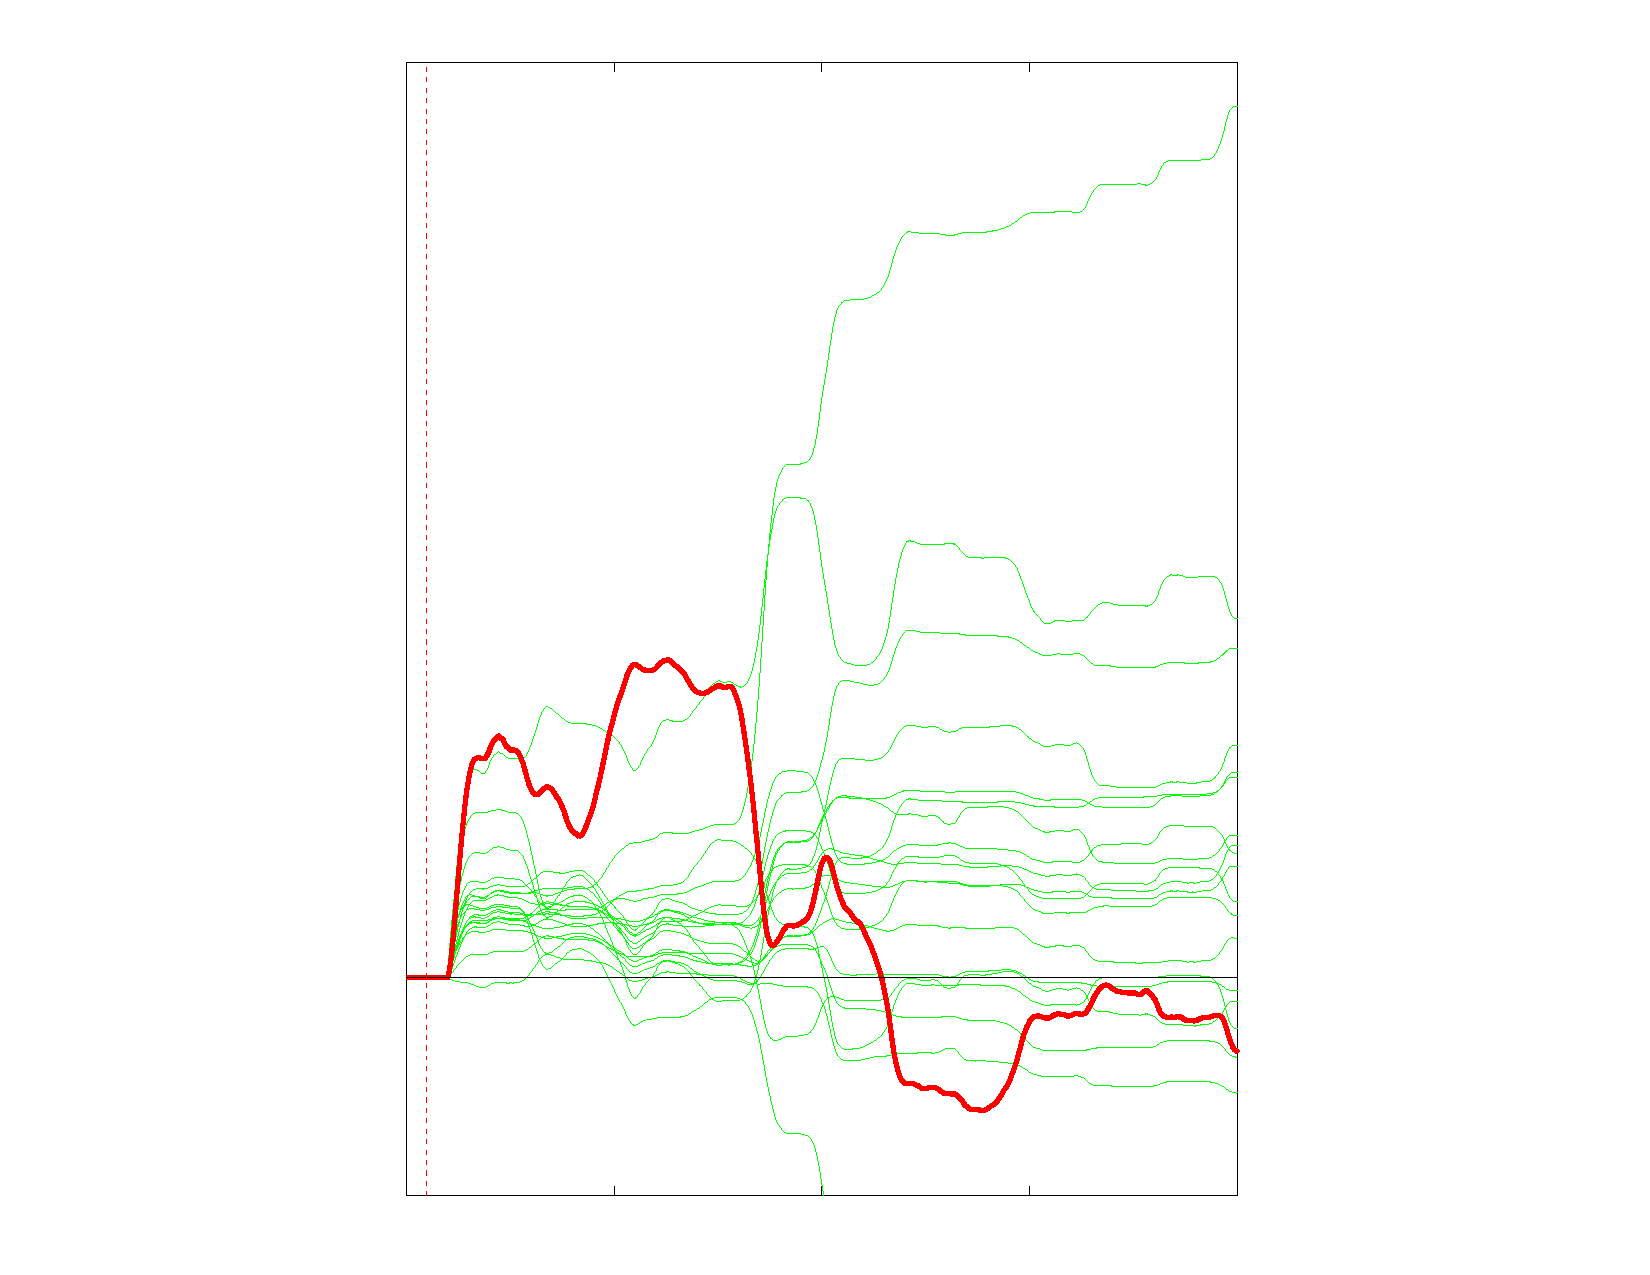
\includegraphics[trim={6.5cm 1cm 5cm 1cm},clip,width=6cm,height=4cm]{img/409-clusterSmallWorld-20-addUniform-40-spike-gaussian-Unobserved-fullKL-ukf-Xhat}};
\node at (0,0) {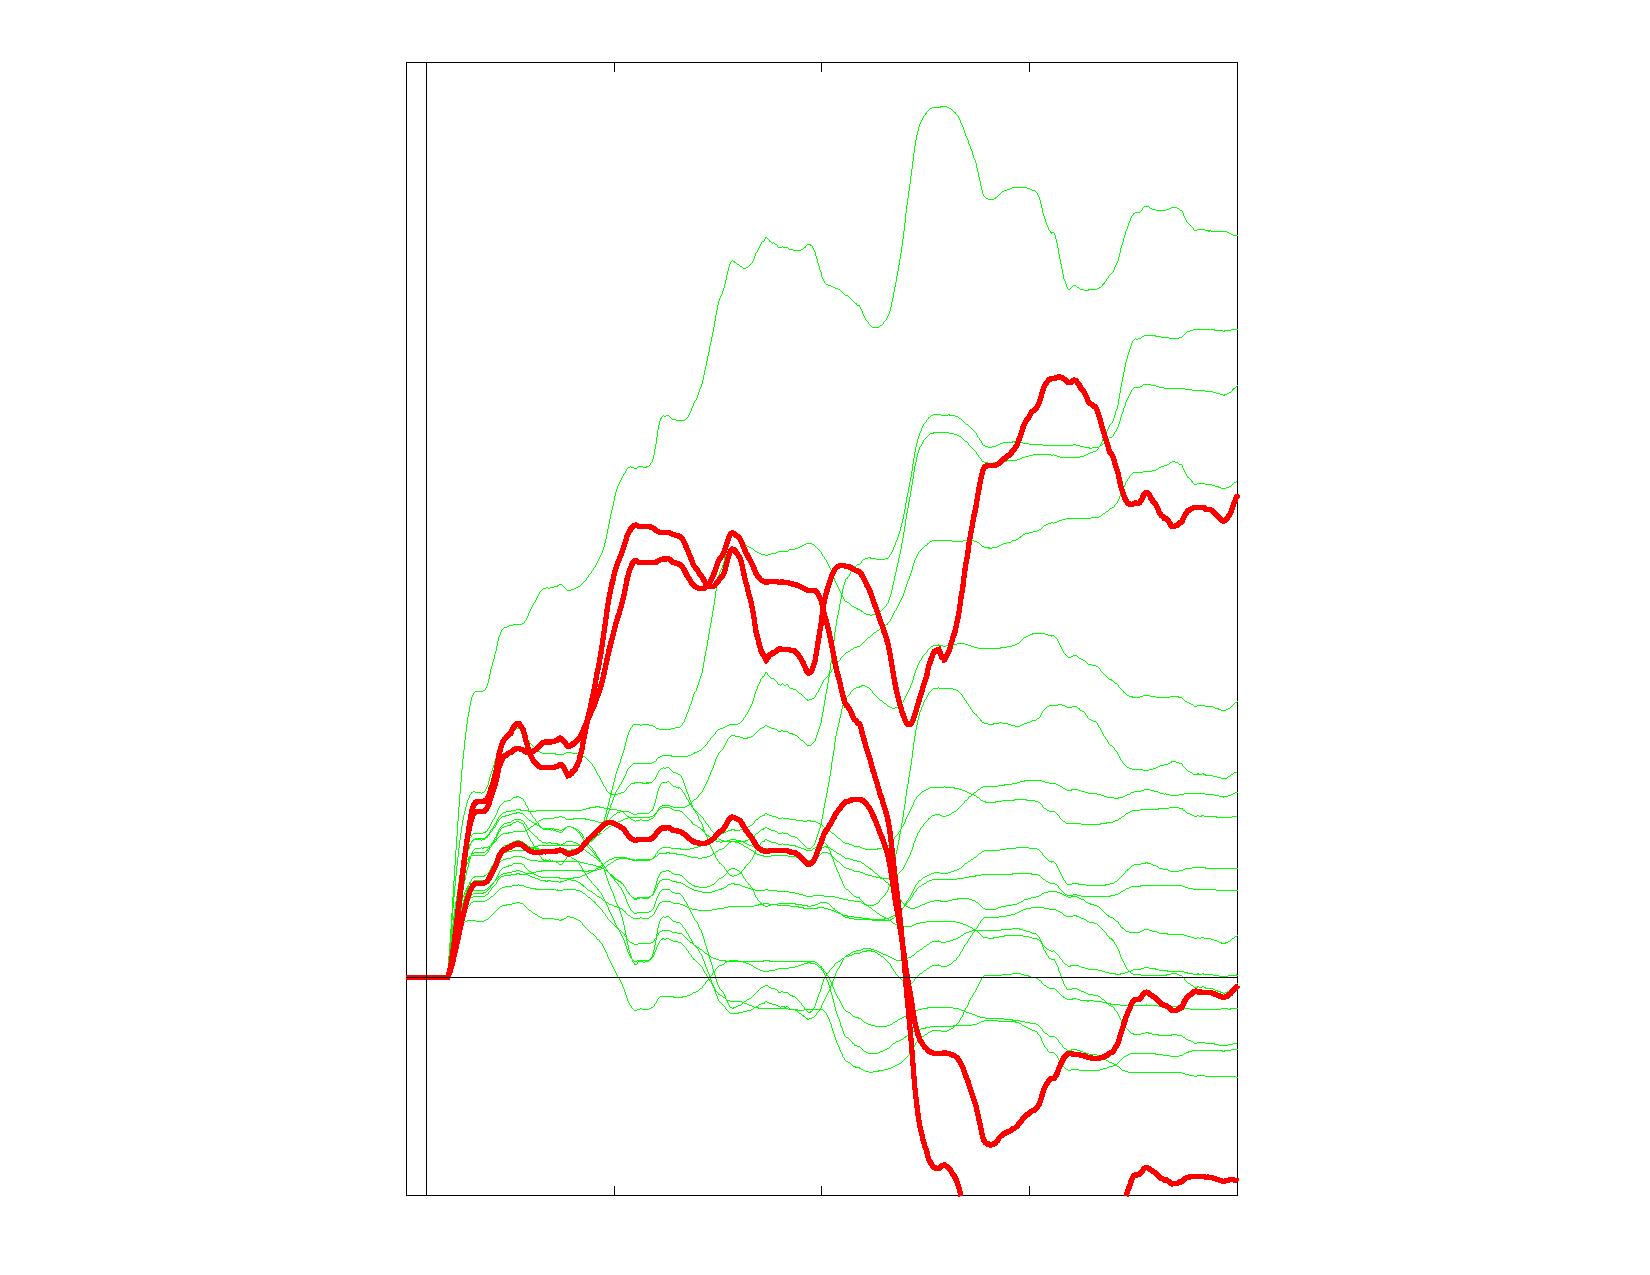
\includegraphics[trim={6.5cm 1cm 5cm 1cm},clip,width=6cm,height=4cm]{img/409-clusterSmallWorld-20-addUniform-40-spike3-gaussian-Unobserved-fullKL-ukf-Xhat}};
\node at (5.5,0) {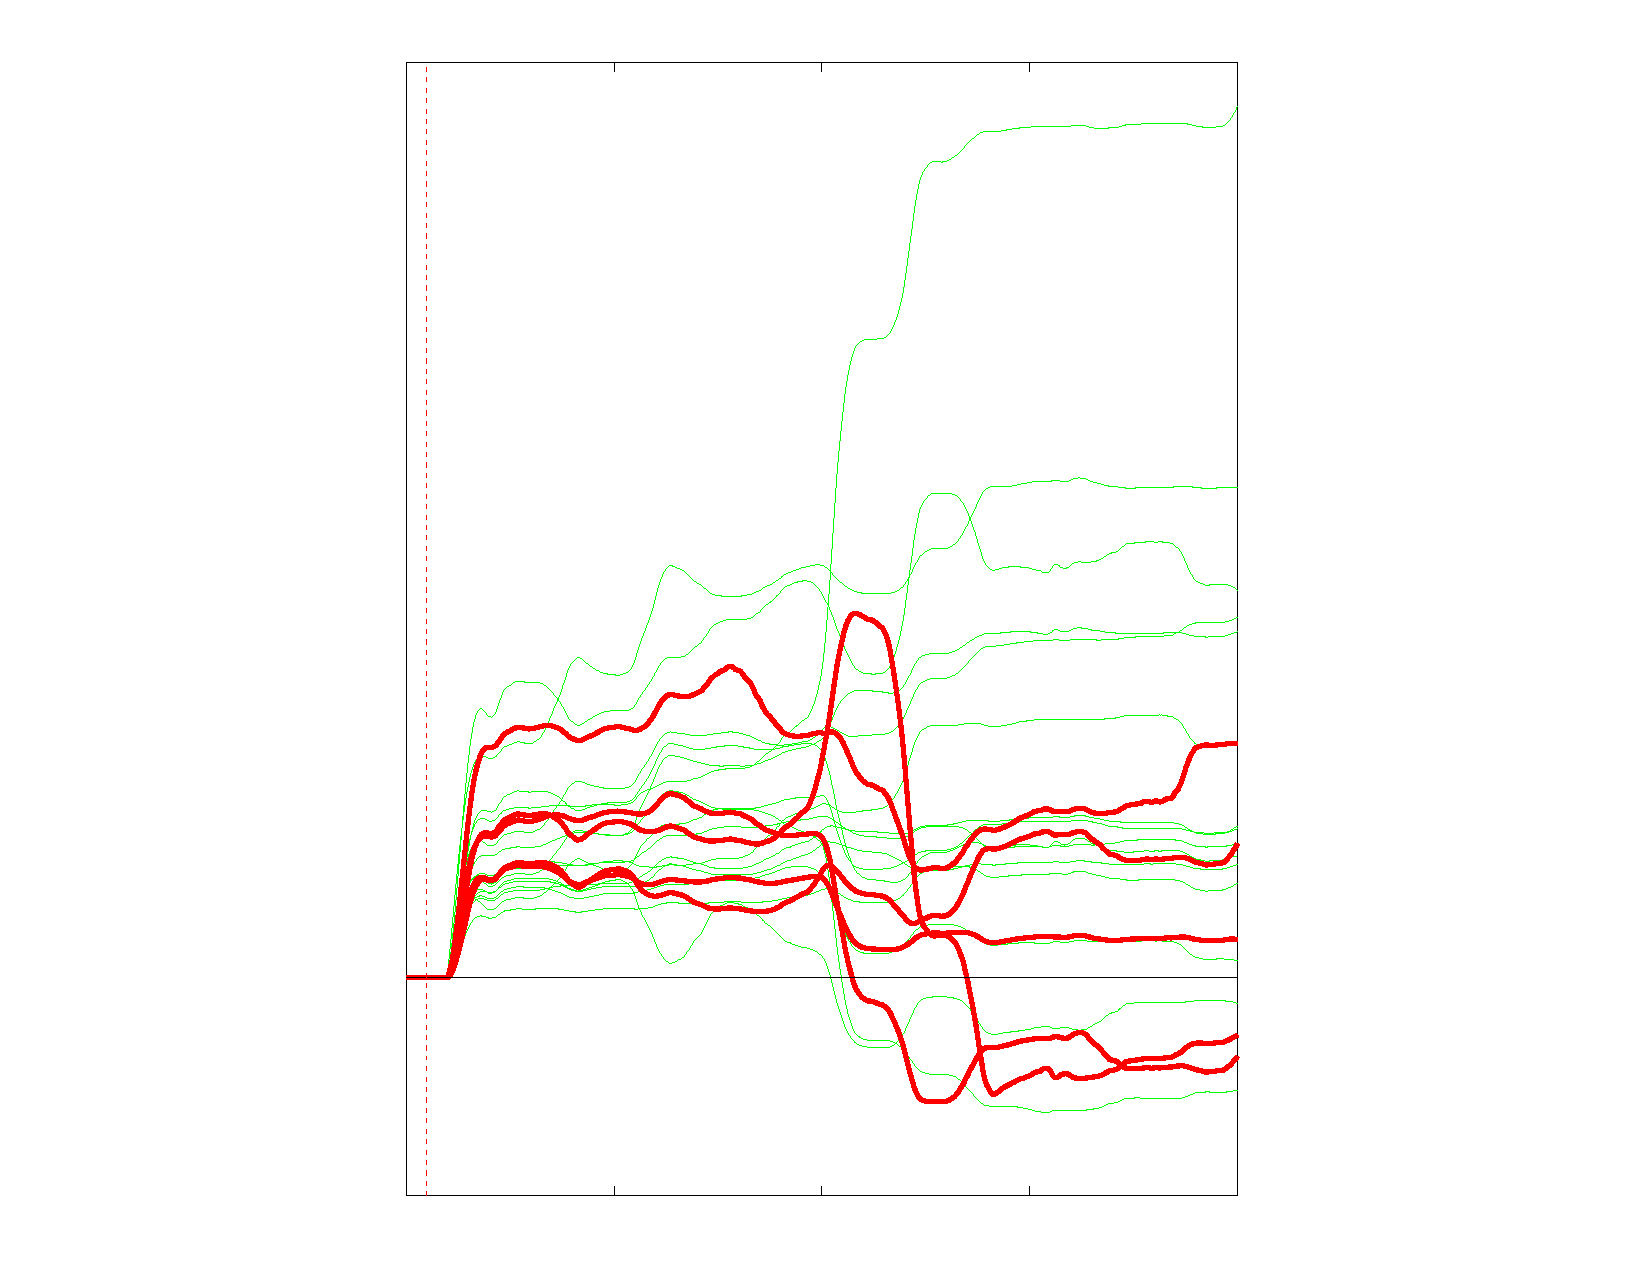
\includegraphics[trim={6.5cm 1cm 5cm 1cm},clip,width=6cm,height=4cm]{img/409-clusterSmallWorld-20-addUniform-40-spike5-gaussian-Unobserved-fullKL-ukf-Xhat}};

\node at (-5.5,4.2) {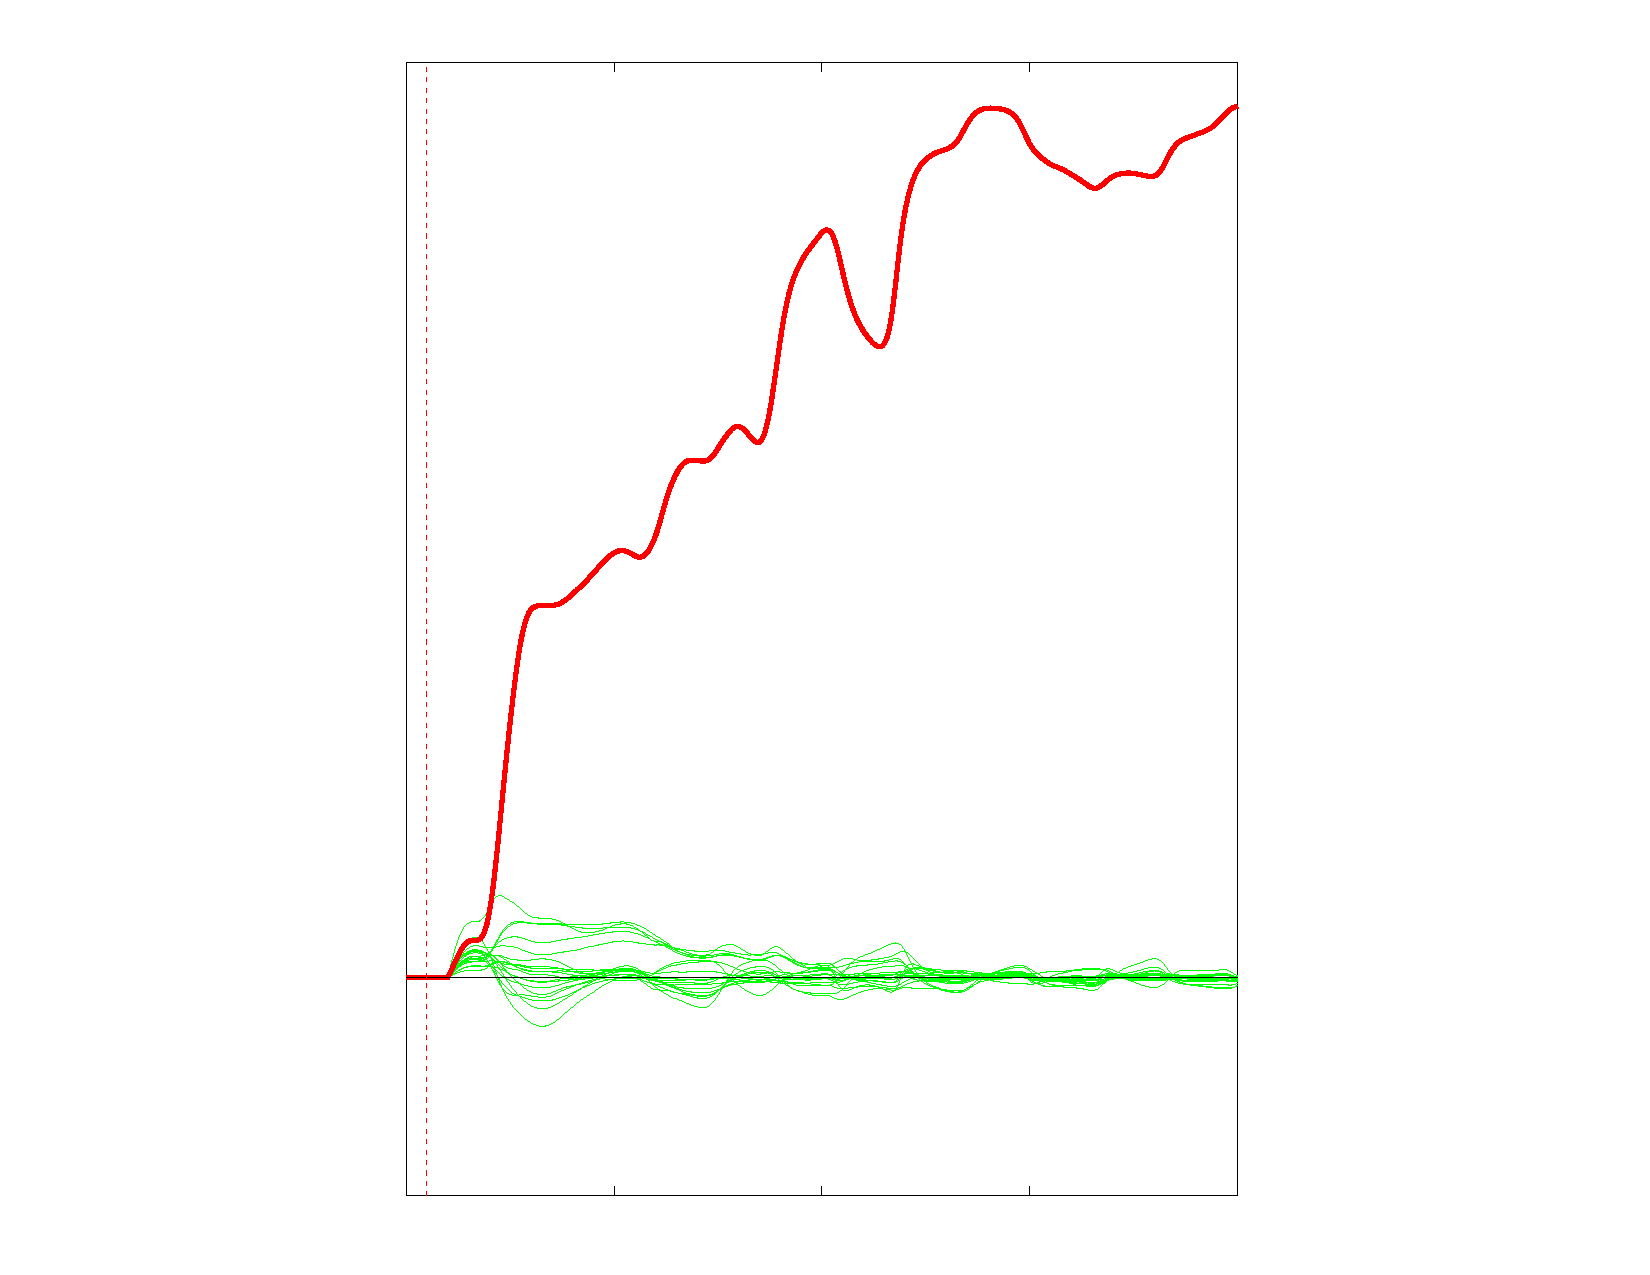
\includegraphics[trim={6.5cm 1cm 5cm 1cm},clip,width=6cm,height=4cm]{img/409-clusterSmallWorld-20-addUniform-40-spike-gaussian-Unobserved-rank1-ukf-Xhat}};
\node at (0,4.2) {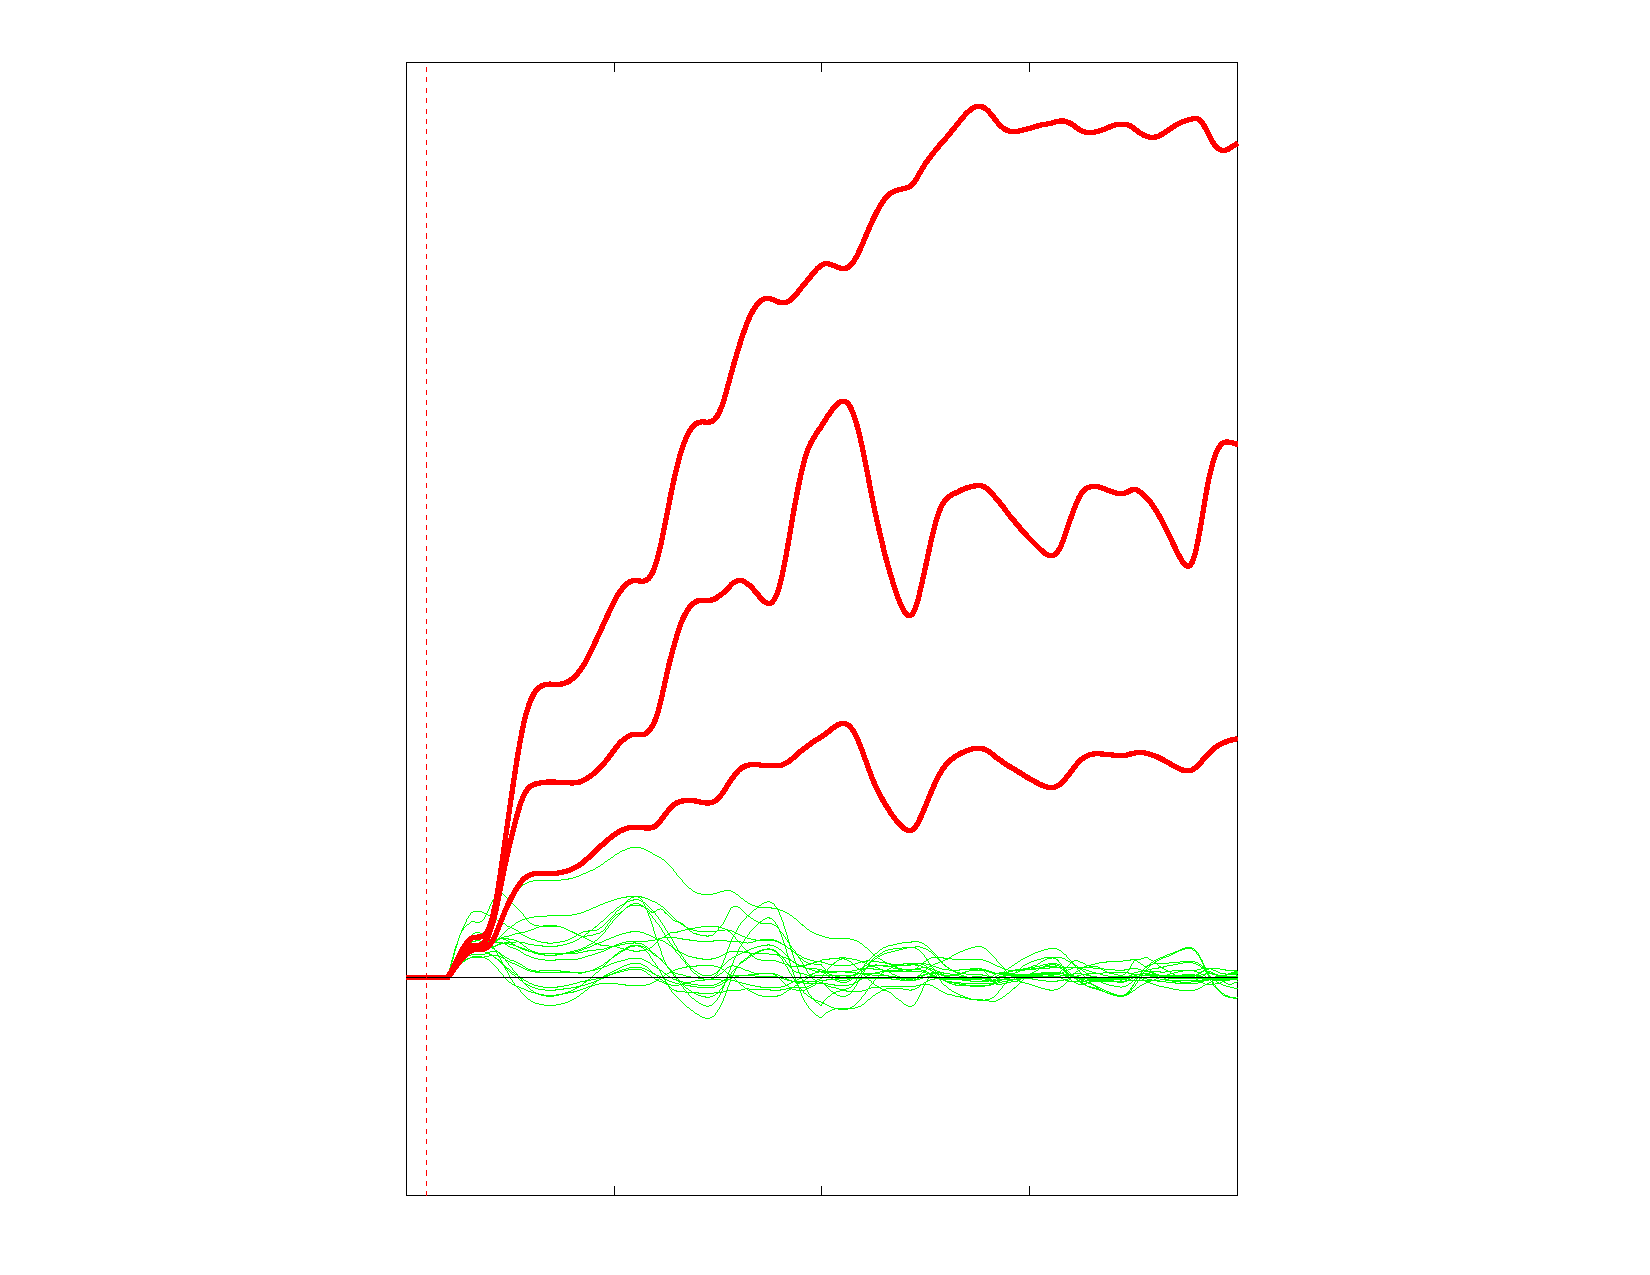
\includegraphics[trim={6.5cm 1cm 5cm 1cm},clip,width=6cm,height=4cm]{img/409-clusterSmallWorld-20-addUniform-40-spike3-gaussian-Unobserved-rank1-ukf-Xhat}};
\node at (5.5,4.2) {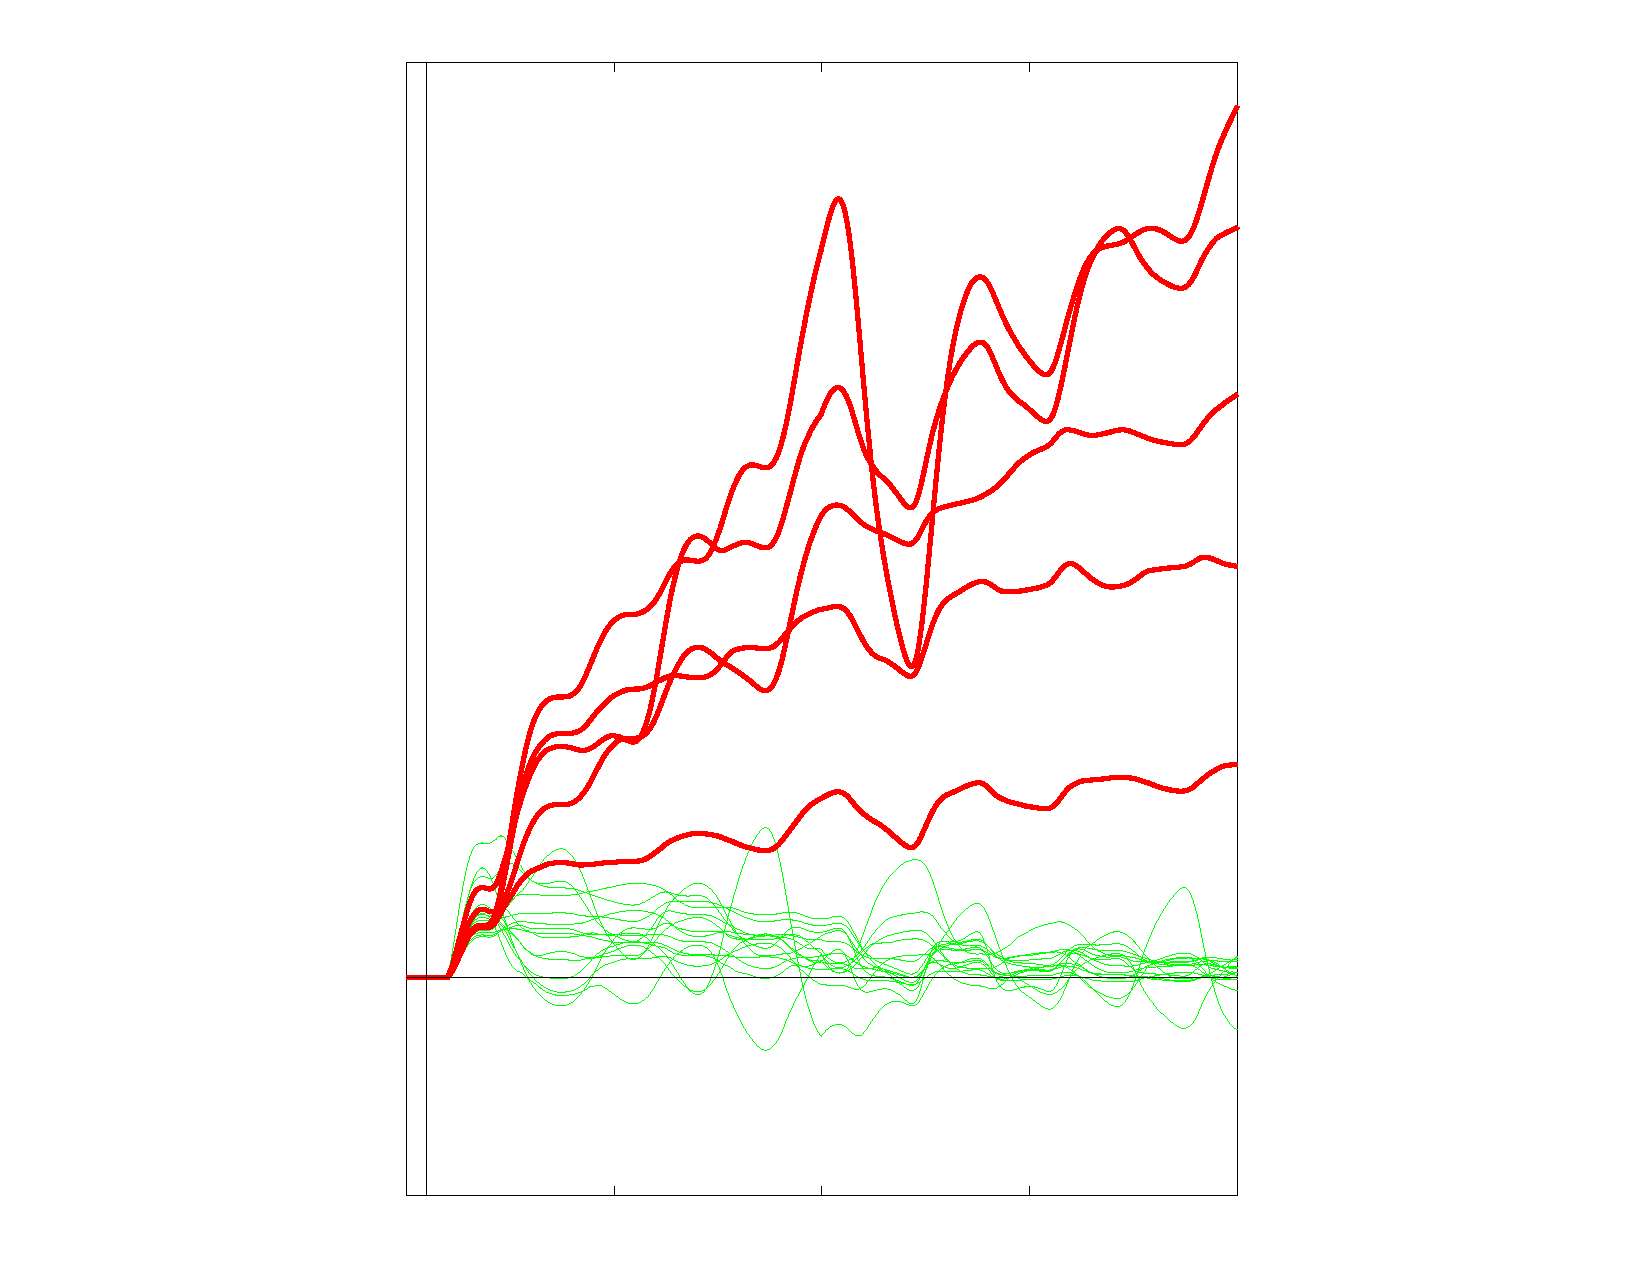
\includegraphics[trim={6.5cm 1cm 5cm 1cm},clip,width=6cm,height=4cm]{img/409-clusterSmallWorld-20-addUniform-40-spike5-gaussian-Unobserved-rank1-ukf-Xhat}};

\node at (-5.5,6.75) {1 attack};
\node at (0,6.75) {3 attacks};
\node at (5.5,6.75) {5 attacks};

\draw (-8.25,-2.5) -- (-6,-2.5);
\draw[->] (-5,-2.5) -- (7.75,-2.5);

\node at (-5.5,-2.5) {time};

\node at (-6.75,1.65) {\color{red} attack initiated};
\draw[->,red] (-7.75,1.65) -- (-8.15,1.65);

\node at (-5,4.25) {\color{red} compromised load};
\draw[->,red] (-6,4.45) -- (-6.25,4.75);

\node at (4.25, 1.5) {\color{darkgreen} uncompromised load};
\draw[->,green] (5.25,1.3) -- (5.5,1.2);
\end{tikzpicture}
\caption{
    Each line in the figures above represents the predicted positive feedback of a particular load bus.
    Buses under attack are drawn in {\textbf{\color{red}bold red}},
    and buses not under attack are drawn in {\color{darkgreen}thin green}.
    For all times $t$ before the attack begins, each bus $i$ has $f_i(t)$ near zero.
    Our method is correctly identifying the attacked buses whenever the red lines are above the green lines.
    In the top row, we see that our rank 1 approximation of $K^{LG}$ provides relatively accurate predictions even when the number of attacks increases.
    In the bottom row, we see that use of the full $K^{LG}$ matrix actually hurts our performance.
    This is because we have too many parameters to estimate.
}
\end{figure*}

%\begin{figure}
%\begin{tabular}{cc}
%\includegraphics[width=0.23\textwidth]{img/4-clusterSmallWorld-100-addUniform-400-spike-gaussian-Unobserved-rank1.eps}
%&
%\includegraphics[width=0.23\textwidth]{img/4-clusterSmallWorld-100-addUniform-400-spike-gaussian-Unobserved-rank1-ukf.eps}
%\\
%time (sec)
%&
%time (sec)
%\end{tabular}
%\caption{
    %(\emph{left})
    %The values of the system states $\x_t$ as a function of time.
    %Each component of $\x_t$ is drawn as a separate line.
    %Before the attack (at time 0.1 sec), all system variables are essentially zero.
    %After the attack, the system is destabilized.
    %(\emph{right})
    %The values of $f_t(i)$ as a function of time.
    %Each value of $i$ is drawn as a separate line.
    %The true attack location is indicated in red.
    %Our method quickly identifies the true location,
    %and the estimate quickly converges to the true value.
    %}
%\label{fig:destab}
%\end{figure}

Our next experiment shows how our predictions scale as a function of the number of attacks.
We repeat the same procedure as above, but add more nonzero entries to $A^p_t$.
The results of 3 and 5 nonzero entries are shown in Figure \ref{fig:numattacks}.
The rank-1 approximation of $K^L$ does fairly well even when the number of attacks increases.
This is surprising because the true $K^L$ matrix has rank equal to the number of attacks.

%\begin{figure}
%\begin{tabular}{cc}
   %\includegraphics[width=0.23\textwidth]{img/4-clusterSmallWorld-100-addUniform-400-spike3-gaussian-Unobserved-rank1-ukf.eps}
%&  \includegraphics[width=0.23\textwidth]{img/4-clusterSmallWorld-100-addUniform-400-spike5-gaussian-Unobserved-rank1-ukf.eps}
%\\
%time (sec)
%&
%time (sec)
%\end{tabular}
%\caption{
    %The values of $f_t(i)$ with 3 attacks (left) and 5 attacks (right).
    %As above, the attack locations are colored in red and non-attack locations are green.
    %In both cases, our method quickly identifies that an attack occurs.
    %In the case of 5 attacks, the rank-1 approximation of $A^p_t$ is not accurate enough to get a correct prediction of the values for all attack locations.
    %Importantly, however, the value of $\alpha_t$ remains a correct attack location.
    %If this bus is isolated, then the system will stabilize.
%}
%\label{fig:numattacks}
%\end{figure}

%Then we apply 1, 3, or 5 attacks to the power grid on random buses.
%The results are shown in Figure \ref{fig:numattacks}.
%As expected, our rank-1 UKF has good accuracy when there is a single attack.
%Somewhat surprisingly, this method continues to work well even when there are multiple attacks.
%The displayed results are for only a single power grid, but the results are qualitatively similar on other power grids as well.

%\begin{figure*}
%\begin{tabular}{ccc}
%\\ 1 Attack
%&  3 Attacks
%&  5 Attacks
%%\\ \includegraphics[width=0.33\textwidth]{img/4-clusterSmallWorld-100-addUniform-400-spike-gaussian-Unobserved-rank1.eps}
%%&  \includegraphics[width=0.33\textwidth]{img/4-clusterSmallWorld-100-addUniform-400-spike3-gaussian-Unobserved-rank1.eps}
%%&  \includegraphics[width=0.33\textwidth]{img/4-clusterSmallWorld-100-addUniform-400-spike5-gaussian-Unobserved-rank1.eps}
%\\ \includegraphics[width=0.3\textwidth]{img/4-clusterSmallWorld-100-addUniform-400-spike-gaussian-Unobserved-rank1-ukf.eps}
%&  \includegraphics[width=0.3\textwidth]{img/4-clusterSmallWorld-100-addUniform-400-spike3-gaussian-Unobserved-rank1-ukf.eps}
%&  \includegraphics[width=0.3\textwidth]{img/4-clusterSmallWorld-100-addUniform-400-spike5-gaussian-Unobserved-rank1-ukf.eps}
%\end{tabular}
%\caption{
    %This figure shows the predicted attack levels on the same power grid (with 100 loads and 100 generators) in three different scenarios.
    %In each scenario, the attack happens at time 0.1 seconds.
    %The only difference between the scenarios is the number of attacks that occurred simulutaneously.
    %In each plot, the values of the estimated $A^p_t$ matrix are plotted over time.
    %Each line in the plot corresponds to a single entry in the matrix.
    %If an entry was actually attacked, then the corresponding line is colored red;
    %otherwise, the corresponding line is colored green.
    %In the left figure, only a single attack occurs.
    %Our algorithm is able to quickly identify the presence of an attack, which bus the attack occurred on, and the strength of the attack.
    %In the middle figure, three attacks occur simultaneously.
    %The algorithm is able to quickly identify the presence of an attack, but has slightly slower convergence to its steady state values.
    %In the right figure, five attacks occur simultaneously.
    %In this case, the algorithm is able to quickly identify the attack, but incorrectly predicts that some of the attacks are introducing negative feedback.
    %This is because our algorithm uses a rank 1 approximation of the $A^p_t$ matrix, but the true attack in this case requires a rank 5 matrix.
    %The closest rank 1 matrix to the attack matrix has negative numbers in the corresponding entries.
%}
%\label{fig:numattacks}
%\end{figure*}

Our last qualitative experiment shows that our UKF method can also detect negative feedback added to the power system.
We repeat the procedure of the first experiment,
but set the value of ${A^p_t}^{(i,j)}$ to $-10$.
Recall that negative values of the $A^p_t$ matrix correspond to negative feedback.
The results are shown in Figure \ref{fig:neg}.
Negative feedback does not destabilize the system,
yet we are still able to detect the feedback.
Previous methods could not differentiate between positive and negative feedback.

\begin{figure}
\begin{tabular}{cc}
\includegraphics[width=0.23\textwidth]{img/4-clusterSmallWorld-20-addUniform-20-spikeNeg-gaussian-Unobserved-rank1.eps}
&
\includegraphics[width=0.23\textwidth]{img/4-clusterSmallWorld-20-addUniform-20-spikeNeg-gaussian-Unobserved-rank1-ukf.eps}
\\
time (sec)
&
time (sec)
\end{tabular}
\caption{
    (\emph{left})
    The values of the system states $\x_t$ as a function of time as in Figure \ref{fig:destab}.
    The negative feedback is added at time 0.1 seconds.
    (\emph{right})
    The values of $f_t(i)$ as a function of time as in Figures \ref{fig:destab} and \ref{fig:numattacks}.
    The predicted value of the added location goes negative and is clearly separated from the rest.
    }
\label{fig:neg}
\end{figure}
\begin{figure}
\end{figure}

\subsection{Quantitative experiments}

For the experiments in this section, we randomly generated 20 different power grids following the same procedure as the previous section.
In each scenario, we use a single attack initiated at time 0.1 seconds.
The goal is to show that our method works on many realistic power grids and not just the special case demonstrated above.

A major strength of our method is that it has essentially no false positives.
We define a false positive to be the detection of an attack when no attack occurred (it does not matter if the value of $\alpha_t$ is correct).
When no attack is underway, the values of $A^p_t$ are typically less than $10^{-6}$.
When an attack is underway, the largest values of $A^p_t$ skyrocket to well above $10^{-1}$.
Therefore, it is easy to set the threshold $\tau$ to avoid false positives.

Next, we evaluate the accuracy of our method.
We define the accuracy at time point $t$ to be the fraction of $\alpha_t$ values that correctly predict the attacked bus.
Figure \ref{fig:accuracy} shows that the longer we wait to declare an attack occurs (i.e. the larger we set $\tau$), the higher our accuracy is.
If we are willing to wait two seconds after an attack begins before taking corrective action,
then we will essentially always be taking corrective action against the attacked bus.
In practice, two seconds is not enough time for an attack to have caused the state values $\x_t$ to exceed their safe operating values.

%The next important measure is the method's accuracy.
%That is, when we identify an attack
%First, we want to emphasize that our method has an essentially zero false positive rate.
%
%For the first experiment, we measured

\begin{figure}
\begin{tabular}{cc}
\begin{turn}{90}
~~~~~~~~~~~~~accuracy of $\alpha_t$
\end{turn}
&
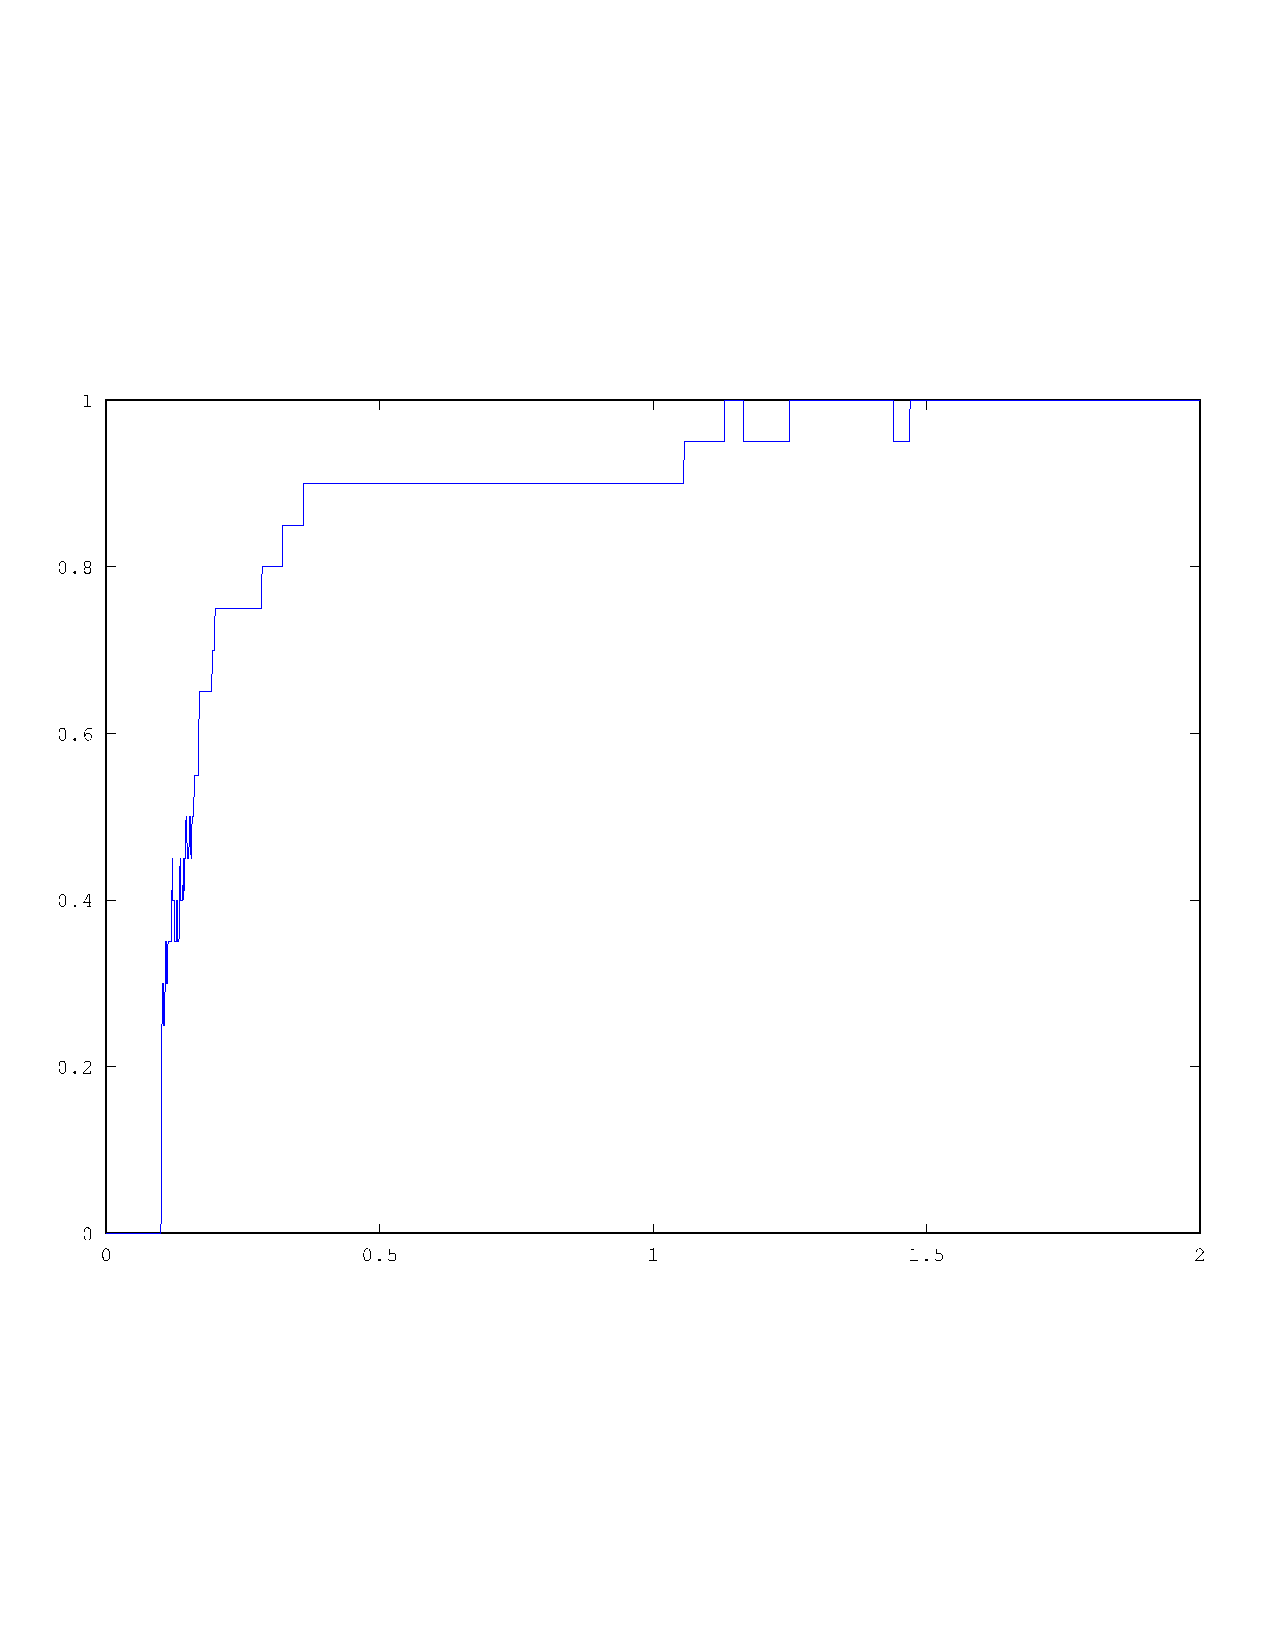
\includegraphics[width=0.4\textwidth, trim= 0 2in 0 2in, clip]{img/clusterSmallWorld-100-addUniform-400-spike-gaussian-Unobserved-rank1-ukf-fraction}
\\
& time
\end{tabular}
\caption{
    Immediately after the attack begins, $\alpha_t$ has modest accuracy.
    Within half a second, $\alpha_t$ has reached 90 percent accuracy.
    By two seconds, $\alpha_t$ is essentially 100 percent accurate.
}
\label{fig:accuracy}
\end{figure}

%\begin{figure}
%\begin{tabular}{cc}
%\begin{turn}{90}
%~~~~~~~~~~threshold
%\end{turn}
%&
%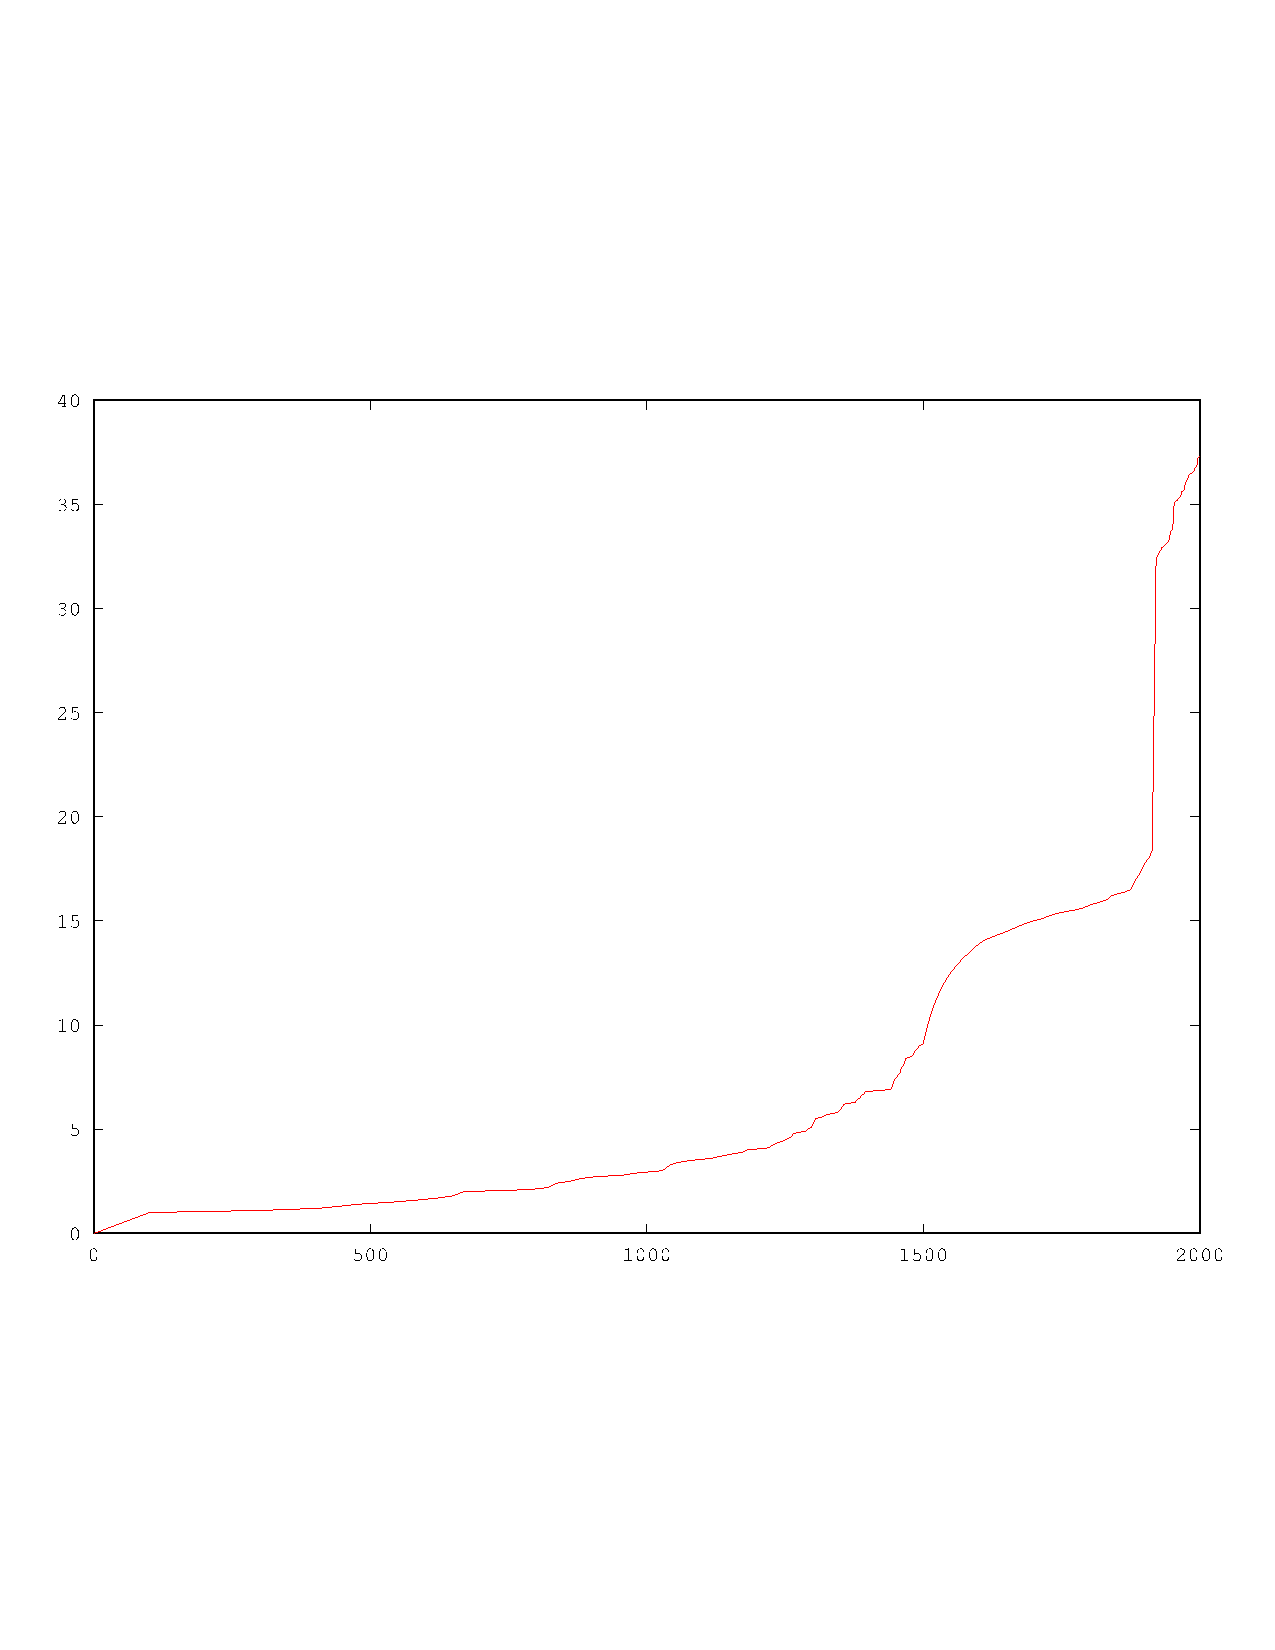
\includegraphics[width=0.4\textwidth, trim= 0 2in 0 2in, clip]{img/clusterSmallWorld-100-addUniform-400-spike-gaussian-Unobserved-rank1-ukf-thresholds}
%\\
%&
%time
%\end{tabular}
%\caption{
    %This plot shows the average time to first detection of an attack as a function of the threshold value.
%}
%\label{fig:threshold}
%\end{figure}

%%%%%%%%%%%%%%%%%%%%%%%%%%%%%%%%%%%%%%%%%%%%%%%%%%%%%%%%%%%%%%%%%%%%%%%%%%%%%%%%

\bibliographystyle{plain}
\bibliography{paper}
\end{document}
